% 公立はこだて未来大学 卒業論文 テンプレート ver1.50
% (c) Junichi Akita (akita@fun.ac.jp), 2003.10.31
% update by N.T.,  2004.11.10
%
\documentclass{funthesis}
%\documentclass[english]{funthesis} % use [english] option for English style

\usepackage[dvipdfmx]{graphicx} % 図(EPS形式)を本文中で読み込む場合はこれを宣言
\usepackage{here}


% この部分に,タイトル・氏名などを書く.
% タイトルなどの定義の始まり
\jtitle{創造活動におけるグループ編成支援ツールの提案\\
--- ユーザー視点を取り入れて ---
}  % 論文の和文タイトル
%
\etitle{Suggestion of group support tool in the design process\\
--- English Subtitle ---
}% 論文の英文タイトル
%
\htitle{Short Title in English}   % ヘッダー用の論文の短縮英文タイトル
%     必ず1行に収まるように英文タイトルを短縮¥¥¥¥¥¥¥¥¥¥¥¥¥¥¥¥

%
\jauthor{田中 康介}     % 氏名(日本語)
\eauthor{Kosuke Tanaka}   % 氏名(英語)
\jaffiliciation{情報アーキテクチャ学科} % 所属学科名(日本語)
\eaffiliciation{Department of Media Architecture} % 所属学科名(英語)
\studentnumber{1015013}   % 学籍番号
\jadvisor{姜 南圭}    % 正指導教員名(日本語)
\eadvisor{Prof. Kang}  % 正指導教員名(英語)
\jdate{2019年1月29日}    % 論文提出日   (日本語)
\edate{January 29, 2019}     % 論文提出年月 (英語)
% タイトルなどの定義の終わり

\begin{document}

%--------------------------------------------------------------------
\maketitle       % タイトルページを作成

%--------------------------------------------------------------------
% 英文概要(250語程度)
\begin{eabstract}
Currently, problems that designers have to deal with are considering the relationship with the users and the society. Therefore, it becomes difficult to find the best answer with the sensitivity and creativity of individual designers.As a result, it is required to organize teams by members with various skills and to conduct creative activities systematically.In the previous studies, results are gotten by distributing human resources in a well-balanced manner.But, it has not been reported what kind of influence the member composition has on creative activities.Consequently, we conducted a survey about group work in creative activities.As a result, most people chose group work rather than personal work for different reasons such as expanding their own vision.In this research, we suggest a web application, named ‘Skill Pentagon’ for organizing more various groups by visualizing the user's skill.
\end{eabstract}

% 英文キーワード(5個程度をコンマ(,)で区切って羅列する)
\begin{ekeyword}
Design Process, Group work, Web application, Creativity
\end{ekeyword}

%--------------------------------------------------------------------
% 和文概要(400字程度)
\begin{jabstract}
現在デザイナーが対処すべき問題は,ユーザや社会との関係性をより丹念に考慮することが 求められるようになり,デザイナー個人の感性や創造性だけでは最適な答えを出すことは難しくなっている.このことから,多種多様なスキルを持つメンバーによってチームを組み,組織的に創造活動をすることが求められている.  先行研究では,様々な要素を利用してグループ編成を行なっている.しかし,グループは実験者が意図して編成しているため,被験者側がどのようなグループなのか把握できない問題がある.そこで,公立はこだて未来大学にて創造活動におけるグ ループワークの現状についてのアンケート調査を行った.その結果,視野が広がるなどの理由から,自分と異なるスキルを持つ人とグループワークを支持する人が大多数であるということが分かった. 本稿ではユーザのスキルを可視化することにより,より多種多様なグループ編成を行うための Web アプリケーションの提案を行う.
\end{jabstract}

% 和文キーワード(5個程度をコンマ(,)で区切って羅列する)
\begin{jkeyword}
デザインプロセス, グループワーク,ウェブアプリケーション, 創造性
\end{jkeyword}

%--------------------------------------------------------------------
\tableofcontents % 目次を作成


% 本文のはじまり
%--------------------------------------------------------------------
\chapter{序論} % 章のタイトル
%\chapter{Introduction} % sample of English style

本章では、本研究における背景と、研究目的について述べる.

% \includegraphics[width=??cm]{hoge.eps} % 図(EPS形式)を読み込む場合

\section{背景} % sectionのタイトル

% 以下に背景,関連する環境,状況,技術に関する概要を記述.

現在デザイナーが対処すべき問題は,ユーザや社会との関係性をより丹念に考慮することが求められるようになり,デザイナー個人の感性や創造性だけでは最適な答えを出すことは難しくなっている.そこで個人の創造性を超えて,多角的な方面からより創造的な解を生み出すために多様な専門性を持つチームによる組織的なデザイン行為のあり方について議論されることが増えてきた\cite{A1}. 石井らは創造性という観点から一般的な創造活動の認知モデルであるジェネプロアモデルの枠組みを適応し,問題解決においてアイデアを検討する段階に限定したうえで,「独立して考える場合と比較して二人で話し合うという協同には効果がある」と示した\cite{A2}. また,Kangは異なる学問や経験,文化を持っている人が集まりグループワークを行うことは,大きな創造性を生み出す潜在能力を持っている\cite{A3}としている.\\
\ これらのことから,自分と異なるスキルや視点を持つ人と共に創造的な作業を行うことにより,自分だけの潜在能力では考えることができなかった成果をあげることがあると考えられる.\\
\ しかし、グループワークにおいて, グループを形成するメンバーによっては、手を抜く学生が生じ、一人に過剰な負荷がかかるなどの問題も指摘されていることもあり\cite{A4}様々なグループ形成方法が議論されているのが現状である.

\section{研究目的}
本研究では創造性とグループワークに着目し,  個人のスキル,情報を可視化し,グループワークをする際により安定し,
グループメンバーが満足するグループを構成するためのツールの提案を行う.
%--------------------------------------------------------------------
\chapter{用語定義}
\section{創造性}
「創造」について日本創造性学会では,「創造とは,人が異質な情報群を組み合わせ統合して問題を解決し,社会あるいは個人レベルで,新しい価値を生むこと」であるとしている\cite{A12}.近藤ら\cite{A13}は創造性の定義についての厳密な指標は見出されていないが,新規性と有用性を含む産物を生み出す態度,プロセス,環境間の相互作用であるということは共通すると考えられているとし,創造性は創造者の内部で完結するものではなく,社会文化的なものであると述べている.\\
\ またKJ法の提唱者である川喜多は創造とは,「発明や発見の能力ではなく,問題解決能力である」または創造性とは,「現状を打破し,常に新しい状態に変えていくことである」と定義し,概念の具現化のため,創造的行為を以下の3点としている\cite{A14} \cite{A15}.(表\ref{souzousei})
\begin{table}[H]
\begin{center}
  \begin{tabular}{|c|p{105mm}|p{10mm}|} \hline
    自発性& その仕事を自発的に行えば行うほど、そこには創造的に言いたいと何かがある\tabularnewline \hline
    モデルのなさ& その仕事をやるのに、こうすればできるに決まっているというモデルとかお手本がなければならないほど創造的で,マニュアル等は全くない仕事である」 \tabularnewline \hline
    切実性&その仕事をやるのことが冗談や酔狂ではなくて,自分にとって切実であればあるほど創造的である.\tabularnewline
    \hline
  \end{tabular}
  \caption{創造的行為}
  \label{souzousei}
  \end{center}
\end{table}


\ そこで本研究の「創造性」は「人が異質な情報群を組み合わせ統合して問題を解決し,創造者内部で完結されることのない,社会あるいは個人レベルで新しい価値を生むこと」とする.

\section{グループワーク}
グループとは典型的には特定の目標や仕事に集中する個人の集まりであると定義される.グループワークとはグループによる目標志向的な活動であり,ソーシャルワークの分野や教育の分野で多くの研究が行われている\cite{A13}.
2つの分野のグループワークの考え方を整理すると,グループワークには個人では達成できない成果をグループによって生み出すことを目的とするものと参加者に何らかの変容をもたらすことを目的とするものがあり,さらに参加者に変容をもたらすことを目的とするものには,参加者個々の学習を目的とするものとチームワークスキルのようなグループ状況における相互作用スキルの育成を目的とするものがあるといえ,メンバー構成や評価基準は表のように整理することができる.\cite{A13}
\begin{table}[h]
\begin{center}
  \begin{tabular}{lll} \hline
    分類& メンバー構成&評価基準\tabularnewline \hline
    学習目的& 学習課題に対する共通の関心や問題 & 
    学習者の学習の程度\tabularnewline
    スキル育成目的&相互作用スキルに対する共通の関心や問題& 
    参加者のスキル獲得の程度\tabularnewline
    成果目的&課題に対する才能,専門性&
    グループによる成果\tabularnewline
    \hline
  \end{tabular}
  \caption{グループワークの分類}
  \label{groupwork}
  \end{center}
\end{table}

本研究のグループワークは成果目的型グループワークとする.



%--------------------------------------------------------------------
\chapter{関連研究}

\section{創造性と協働活動}

\subsection{創造性課題における協働性の効果について} % subsectionのタイトル
村谷・阪田\cite{A10}は発散的なアイデア生成を要する課題において,個人で取り組むよりも,複数人で取り組んだ方が,創造性の質が高まるかを検証した.検証は個人と同性の2人組に割り振り行われ,2人組みの方が,創造性の質が高まることが示された.また男性と女性では協働性の効果のあらわれ方が異なることが示された.西本らは\cite{A11}は協働作業において,女性はグループ内の親和性を重視する一方で,男性はよりよい作品を完成させることを重視することを示した.検証結果と照らし合わせ,女性はペアになると親和性を重視することにより,会話を和ませようと独創性の高いアイデアを産出するようになり,男性はペアになるとよりよい作品を完成することに意識が向くことにより,より実用性の高いアイデアを産出するようになると考察した.
\section{グループ編成}

\subsection{DTMPメソッドを用いたグループ編成システム}

相島・塚原・植木・杉浦\cite{A5}は学習プロセス方法論であるDTMPメソッドをユーザのふるまいに当てはめ,人的リソースを配分する手法を提案し,ウェブアプリケーションを実装,グループ学習において検証を行った.DTMPメソッドとは,  DTMPの各系統の能力について以下の表のように定義したものである(表\ref{DTMP}).

\begin{table}[h]
\begin{center}
%\scalebox{0.8}[1]{
  \begin{tabular}{|c|p{25mm}|p{105mm}|} \hline
    D & Design & 創造的な本質を理解し,創造活動を実践できる能力\tabularnewline \hline
    T & Technology & 
    創造的活動を支えるデジタルメディア関連の技術を理解・活用できる能力\tabularnewline \hline
    M &Management & 
    創造的デザインプロセスを管理できる能力\tabularnewline \hline
    P &Polisy &
    創造的活動の成果を戦略的に活用でき,創造的プロセスを取り巻く政策を理解できる能力\tabularnewline
    \hline
  \end{tabular}
 % }
  \caption{DTMPメソッドの定義}
  \label{DTMP}
  \end{center}
\end{table}


\ ふるまいはユーザの潜在的な特性を反映しており,DTMP系統の特性を対応づけることにより,個人が持つDTMP特性を抽出できる.\\
\ 抽出した各DTMP特性を元にメンバーを均等に分配し,2ヶ月間のグループワークを行なった.
\ 検証を行った結果,人的リソースのバランス良い配分という観点では効果を認めることができたが,DTMPメソッドの各特性が持つ能力や傾向を確認することはできなかった.

\subsection{ソフトウェア開発グループ演習のためのチーム最適化支援}
橋浦・桑原・秋・石川・山下・古宮\cite{A6}はソフトウェア開発におけるグループ内の役割をリーダー,設計担当,コーディング担当,品質管理担当に分け,それぞれに必要な適正を成績から代用し,遺伝的アルゴリズムを使用してチーム編成を行う手法を提案した.
\begin{table}[h]
\begin{center}
  \begin{tabular}{lll} \hline
    役割(Y) & 適正 & 代用適正の例\tabularnewline \hline
    リーダ & PM能力 & プロジェクトマネジメントに関する問題の成績\tabularnewline
    設計担当 &分析・設計能力 & 
    ソフトウェア設計に関する問題の成績\tabularnewline
    コーディング担当&プログラミング能力 &
    プログラミングに関する問題の成績\tabularnewline
    品質保証担当&品質管理能力 &
    ソフトウェアテスト技術に関する問題の成績\tabularnewline
    \hline
  \end{tabular}
  \caption{役割 - 適正 - 代用適正の関係(例)}
  \label{適正}
  \end{center}
\end{table}
ソフトウェア開発グループ演習において検証を行った結果,学習者の満足度が上がったことと,チーム間の成果物のバラつきが軽減されたことから,ソフトウェア開発演習のための最適なチーム編成が実現できていることを確認した.


\subsection{学習者の思考特性に着目したグループ形成支援の方法}
井上・埴生は\cite{A7}組織最適編成法理論のひとつであるFFS理論(FIve Factors and Stress Theory)
\cite{A8}を用いて,学習者の特性,すなわち,人の個性や潜在能力傾向に着目した協調学習のためのグループ形成方法についての検討を行なった.
\ FFS理論とは,A.凝縮性,B.受容性,C.弁別性,D.拡散性,E.保全性の5つの因子とストレス値をチェックリストによって計量し,A,B,C,D,E因子の計量値から4種類のパーソナリティタイプ(リーダーシップ,マネジメント,タグボート,アンカー)に分類し、各因子がストレス状態によって表出される特徴を(表\ref{FFS})のように示したものである\cite{A9}.
\begin{figure}[h]
 \centering
   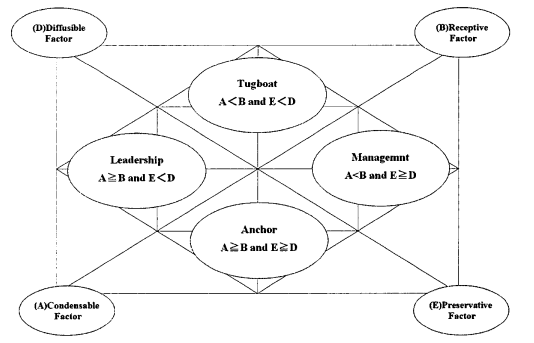
\includegraphics[width=100mm]{figures/FFS.png}
 \caption{パーソナリティタイプの分類}
 \label{FFS}
\end{figure}

\begin{table}[h]
\begin{center}
  \begin{tabular}{lll} \hline
    状態 & ポジティブ反応 & ネガティブ反応\tabularnewline \hline
    A 凝縮性& 規範的,指導的 & 
    独善的,支配的\tabularnewline
    B 受容性 &肯定的,養育的 & 
    介入的,自虐的\tabularnewline
    C 弁別性&分析的,論理的 &
    機械的,詭弁的\tabularnewline
    D 拡散性&創造的,活動的 &
    衝動的,破壊的\tabularnewline
    E 保全性&順応的,協調的 &
    追随的,妥協的\tabularnewline
    \hline
  \end{tabular}
  \caption{各因子のストレス状態における特徴}
  \label{FFS理論}
  \end{center}
\end{table}

\begin{table}[h]
\begin{center}
  \begin{tabular}{lll} \hline
    Personality Type &  コンピテンシー\tabularnewline
   Leadership(LD)& 組織の先頭に立って変革を進める力  \tabularnewline
    Management(MG) & 取り巻く環境を判断しながら継続的に改善する力 \tabularnewline
    Tugboat(TG)& 環境の変化を捉えリスクに挑戦していく力\tabularnewline
    Anchor(AN)&リスクヘッジしながら手続き通りに着実に実行する力 \tabularnewline
    \hline
  \end{tabular}
  \caption{パーソナリティタイプとコンピテンシー}
  \label{FFS理論2}
  \end{center}
\end{table}

FFS理論で各因子を抽出したうえで,グループでの協調学習場面を想定し,創造性,効率性を対立軸として設け,4人のチーム編成を行なった(表\ref{FFS理論3}).

\begin{table}[h]
\begin{center}
  \begin{tabular}{ll} \hline
    創造性を重視したグループ編成\tabularnewline \hline
   1. 補完型グループ& 異質な型のメンバーで構成  \tabularnewline
   2. 意見発散型グループ & LM,AN,TG,TGタイプのメンバーで構成 \tabularnewline
    3. アイデア型グループ& 全員TGタイプのメンバーで構成\tabularnewline \hline
    効率性を重視したグループ編成 \tabularnewline \hline
    4. 同質型グループ& TGタイプを除く同質タイプのみのメンバーで構成  \tabularnewline
    5. 意見収束型グループ & LM,ML,ANタイプとTGタイプ以外のメンバーで構成 \tabularnewline
    6. リーダー主導型グループ&LMタイプが一人とLMタイプ以外の同質メンバーで構成\tabularnewline
    \hline
  \end{tabular}
  \caption{グループ編成}
  \label{FFS理論3}
  \end{center}
\end{table}

チーム編成を行い,学習者が活発に意見交換する創造的な学習活動を意図し,映像分析のグループワークを行なった.補完型グループについて,オブジェクトシーケン図による分析を行なった結果,継続的に相補的に意見交換が行われていることからグループ形成が有効であったと示唆した.



\section{関連研究まとめ}
本章では関連研究を「創造性と協調活動」,「グループ編成」に分けて説明した.「創造性と協調活動」における関連研究では,1人で創造的な活動を行うよりもペアで行った方が良いことが証明され,さらに男女の組み合わせなどにもよって協調活動の効果が変わっていくことが明らかとなった.「グループ編成」における関連調査を以下の表のようにまとめることができる.また表\ref{関連まとめ}DTMPメソッドを用いたグループ編成システムを「研究1」,ソフトウェア開発グループ演習のためのチーム最適化支援を「研究2」,学習者の思考特性に着目したグループ形成支援の方法を「研究3」としている.
\begin{table}[h]
\begin{center}
  \begin{tabular}{llll} \hline
    研究名 & 編成方法 & 自動生成 & 目的\tabularnewline \hline
    研究1& DTMPメソッド & × & 学習誤差を減らす\tabularnewline
    研究2&学生の成績 &◯&成果の安定\tabularnewline
    研究3&× & 効果の実証\tabularnewline
     \hline
  \end{tabular}
  \caption{関連研究まとめ}
  \label{関連まとめ}
  \end{center}
\end{table}



\ 以下のことにより,グループ自動生成機能を行なっている研究が少ないことと,すべてのグループ編成のシステム自体が教育者目線で作られており,ユーザである学習者に伝わっていないことがわかる.そこで本研究ではグループを自動で生成し,その上でグループ情報を可視化することで,ユーザの視点を取り入れたシステムを提案する.
%--------------------------------------------------------------------
\chapter{グループワークの現状と個人の認識に関する調査}

グループ編成ツールの作成にあたり,  グループワークの現状を把握することを目的に調査を行なった.本章では,  調査の方法と目的,  結果,  考察について述べる.
\section{目的}

より多種多様なスキルを持つメンバーによるグループを構成するツールを制作するため,グループワークの現状を調査する.現状を把握することによって,問題を解決する方法を考える.

より安定しグループを構成するツールを制作するため,グループワークの現状を調査する.現状を把握することによって,問題を解決する方法を考える.


\section{調査方法}

本調査は,2018年6月27〜28日に,グループワークが多く行われている公立はこだて未来大学の18〜24歳の大学生,61名(男性49名, 女性12名)を対象に行われた.Googleフォームを用いて作成したアンケートを,回答者にメールにて送信し,回答してもらった.
\begin{figure}[H]
 \centering
   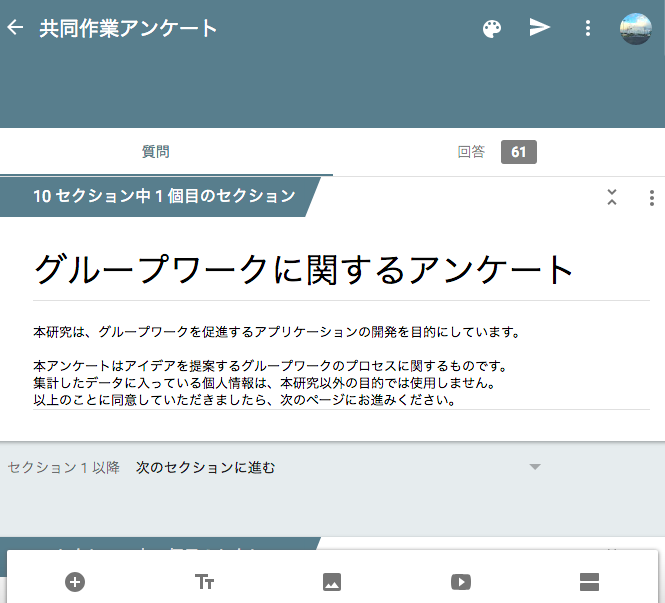
\includegraphics[width=100mm]{figures/groupwork1.png}
 \caption{Googleフォーム画面の一部}
 \label{fig:model}
\end{figure}


\subsection{質問内容}

1問目は,グループワークを通して新しいアイデアを考えたことがあるか.2問目は,新しいアイデアを考える際に良い結果が得られるのは個人ワーク,グループワーク,どちらでもないを選択,またその理由を記述してもらった.3問目は,初対面の人とグループワークをしたことがあるかを選択してもらった.4問目は,初対面の人とグループワークをする際に,その人の情報をあらかじめ知りたいと考えるかを選択,またその人の何を知りたいか記述してもらった.5問目は,グループで作業する際に自分と異なるスキルを持つ人と活動したいかを選択,またその理由を記述してもらった.6問目は,今までグループワークで困った経験はあるかを選択,またその理由を記述してもらった.


\section{調査結果}

アンケート調査の結果,全回答者61名のうち59名(96.7\%)がグループワークを通じて,何らかのアイデアを考えた経験があると回答した.グループワークをした経験がある59名のうち,50名(84.7\%)が新たなアイデアを考案する際に良い結果が得られるのはグループワーク,6名(10.2\%)がどちらでもない,3名(5.1\%)が個人ワークであると回答した.
(図\ref{graph0})
\begin{figure}[H]
 \centering
   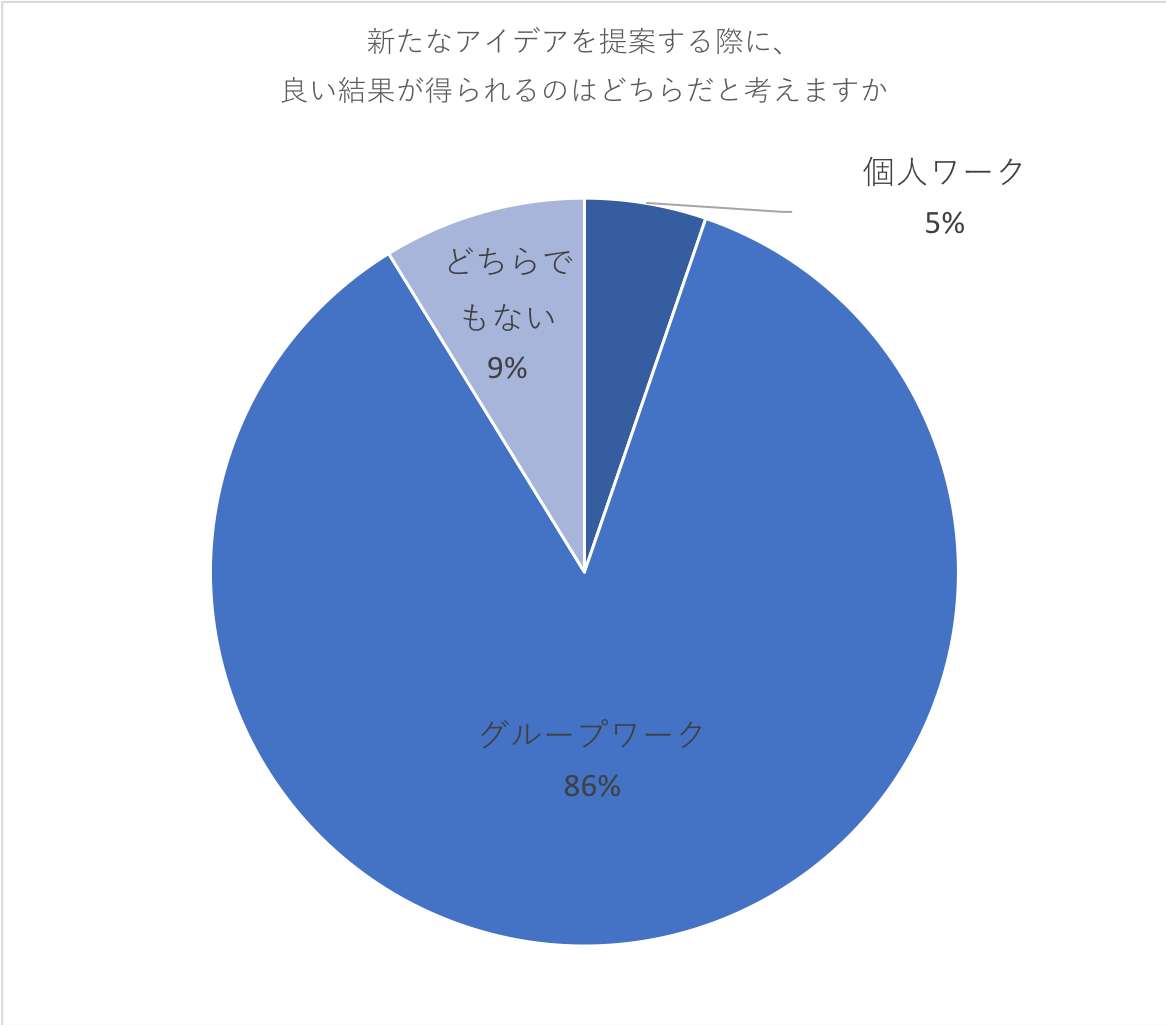
\includegraphics[width=100mm]{figures/en1.png}
 \caption{支持をするのはどちらか}
 \label{graph0}
\end{figure}

\ グループワークを選んだ理由の記述を「様々な意見が得られる」「自分の視野が広がる」「意見を客観駅に見ることができる」「刺激をもらえる」「効率が上がる」の5つに分類した(図\ref{graph1}).
\begin{figure}[H]
 \centering
   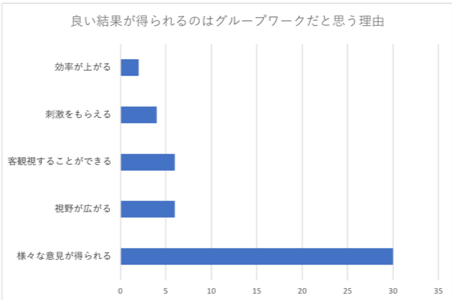
\includegraphics[width=100mm]{figures/graph1.png}
 \caption{グループワークを支持する理由}
 \label{graph1}
\end{figure}

個人ワークを選ぶ理由として,「個人のほうが作業がはかどるから」などの意見などが得られた.どちらでもないを選ぶ理由として「両者に利点があると思うから」という意見などが得られた.
グループワークをした経験がある59名のうち,58名(98.3\%)が初対面の人とグループワークをした経験がある,1名(1.7\%)がないと回答した.
初対面の人とグループワークをしたことがあると回答した58名のうち,28名(48.3\%)が初対面の人の情報をあらかじめ知りたい,21名(36.2\%)がどちらでもない,9名(15.5\%)が知りたいと思わないと回答した 
初対面の人の情報をあらかじめ知りたいと回答した21名のうち,23名が初対面の人の得意分野,22名が性格,14名が趣味,9名が学校・職場,4名が生い立ち,5名がその他と回答した(図\ref{graph2}).

\begin{figure}[H]
 \centering
   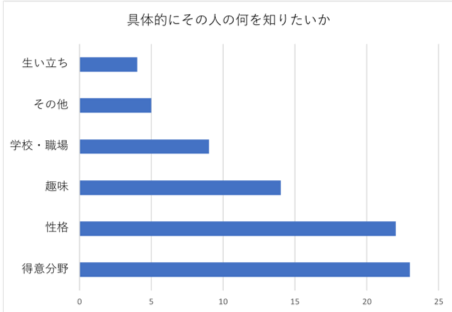
\includegraphics[width=100mm]{figures/graph2.png}
 \caption{具体的に何を知りたいか}
 \label{graph2}
\end{figure}

グループワークをした経験がある59名のうち,57名(96.6\%)がグループワークを行う際に自分と異なるスキルを持った人と活動したい,2名(3.4\%)がどちらでもない,0名が活動したいと思わないと回答した.グループワークを行う際に自分と異なるスキルを持った人と活動したいと回答した57名のうち,活動したいと思う理由の記述データを「視野が広がる,成長できる」「作業の幅が広がる」「作業の効率が上がる」「その他」の4つに分類した.(図\ref{graph3})

\begin{figure}[H]
 \centering
   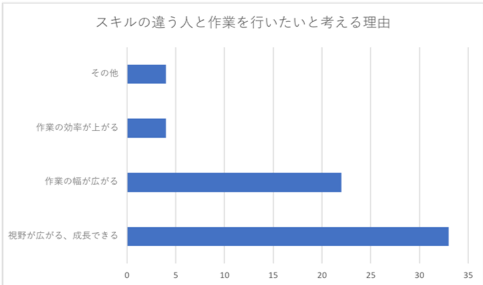
\includegraphics[width=100mm]{figures/graph3.png}
 \caption{スキルの違う人と作業をしたい理由}
 \label{graph3}
\end{figure}

グループワークをした経験がある59名のうち,50名(84.7\%)が今までグループワークをしていて困った経験がある,9名(15.3\%)が経験はないと回答した.グループワークで困った経験があると回答した50名の困った内容を「コミュニケーション」「意見の対立」「管理」「人間関係」「その他」の5つにカテゴリー分けて分類した.(図\ref{graph4})

\begin{figure}[H]
 \centering
   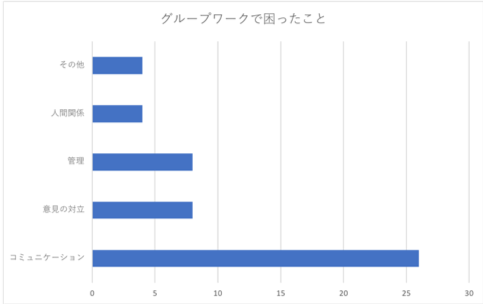
\includegraphics[width=100mm]{figures/graph4.png}
 \caption{グループワークで困ったこと}
 \label{graph4}
\end{figure}


\section{考察}

アンケート調査の結果から,グループワークを経験したことがある87\%が,知識の幅や視野が広がるなどの理由から,新たなアイデアを考案するプロセスでは良い結果が得られるのはグループワークであると認識していることが分かる.また,ほぼ同様の理由で96.6\%がグループワークで自分と異なるスキルを持った人と活動したいと考えていることと,82.1\%が初対面の人の知りたい情報として得意分野をあげている.これらのことから,回答者がグループワークに求めているものはアイデアの幅が広がることや,自分の持っていないスキルを持つ人と行動をすることで視野が広がることであると考えられる.\\
\ しかしグループワークを経験したことがある84.7\%が,知識,価値観の違いからコミュニケーションが進まなかった経験や意見の対立,グループの管理,人間関係などから,グループワークをしていて困った経験があると回答している.意見や価値観,知識の違いは視野を広げる可能性があるが,異なる背景を持つ人を理解する努力をしなければ,人と人が衝突し,逆にアイデアが決まらないことや,作業が進まなくなることが考えられる.
\ 初対面の人とグループワークをしたことがある52.7\%が,初対面の人とグループワークをする際に事前に情報を知りたいと思わない,どちらとも言えないと回答していることから,事前に初対面の人の情報を得ることに関しては消極的であることがわかる.\\
\ また事前に知りたい情報のうち性格と答えた人が78.6\%,趣味と答えた人が50\%であり,それらを高い割合で求めていることと,98.6\%が自分とスキルの異なる人と作業をしたいと考えていることから,知識やスキルに関しては自分と違うものを求めている

%--------------------------------------------------------------------
\chapter{システムの提案}
アンケート調査の結果とその考察から,大多数の人が自分と異なるスキルを持つ人と活動したいと考えていることが分かった.そこで,個人の得意分野にフォーカスをあてて,自分のスキルのデータを可視化し,グループで共有するWebアプリケーションの制作を行なった.

\section{提案コンセプト}
アンケート調査の結果からアイデアが広がる,自分の視野が広がるなどの理由からグループワークが支持されていることがわかった.
本研究の目的は個人のスキル、情報を可視化し、グループワークをする際に、より多種多様なスキルを持つメンバーによってグループを構成するためのツールを作成することである.そこで個人が持つスキルを平等に分配することでグループを作成し,作成したグループ内でグループメンバーのスキルを可視化するWebアプリケーションを提案する.可視化することで,グループメンバーへの理解やコミュニケーションの促進など,互いの理解が深まるの可能性が示唆される.またスキルの可視化はレーダーチャートを用いる.スキルの可視化以外にも自分の情報を入力し,メンバーに共有する機能も作成する.
\ 先行研究では教育者視点でのみのグループ配分をしており,グループワークをする側の視点に立っていない.そこで本システムでは可視化することでユーザー側の視点も導入し,メンバーの相互理解を促進することを目指す.
\section{開発環境}
ここでは開発環境の説明をする.開発環境は以下の通りである.
\begin{table}[h]
\begin{center}
  \begin{tabular}{cll} \hline
    フロントエンド & Vue.js(JavaScript)  \tabularnewline
    バックエンド& Firebase\tabularnewline
    チャート &vue-chartjs \tabularnewline
    \hline
  \end{tabular}
  \caption{開発環境}
  \label{開発環境}
  \end{center}
\end{table}

\subsection{Vue.jsとは}
本システムはプログラミング言語JavaScriptのフレームワークであるVue.jsを採用した.Vue.jsの公式サイトでは
「Vueはユーザーインターフェースを構築するためのプログレッシブフレームワークです。他の一枚板なフレームワークとは異なり、Vue は少しずつ適用していけるように設計されています。モダンなツールやサポートライブラリと併用することで、洗練されたSingle Page Applicationの開発も可能です。」\cite{A16}と説明している.\\
\ 本システムにVue.jsを採用したのは,Single Page Application(以下SPA)を作成できるからである.SPAのシステムを作成することでブラウザによる更新を行わずにコンテンツの切り替えを行うことができ,ユーザー体験を大きく向上させることができる.なおバージョン2.9.6を使用している.
\subsection{Firebaseとは}
Firebaseとはアプリケーションのデータストレージ,ユーザー管理などのバックエンドサービスを提供することで開発者がクライアントサイドの開発に集中することができる,Google社が提供しているBaaS(Backend as a Service)である.\\
\ Firebaseを採用した理由は,バックエンドの実装を容易にすることができる点と高速な非同期通信をすることができる点である.Firebaseを用いることで,より高速なデータ通信を行うことができ,ユーザー体験を向上させることができる.またバージョン6.1.1を使用しており,使用しているFirebaseの機能は以下である(図\ref{Firebase}).

\begin{table}[h]
\begin{center}
  \begin{tabular}{lll} \hline
  機能名&使用用途\tabularnewline \hline
    Firebase Authentication& ユーザー認証  \tabularnewline
    Firebase Hosting&ホスティング機能\tabularnewline
    Realtime Database &データーベース \tabularnewline
    \hline
  \end{tabular}
  \caption{使用しているFirebaseの機能}
  \label{Firebase}
  \end{center}
\end{table}


\subsection{vue-chartjsとは}
vue-chartjsとは,JavaScript上で折れ線グラフ,棒グラフ,レーダーチャートなど6種類のグラフをアニメーション付きで描写することができるChart.jsをVue.jsに適用させたライブラリである.vue-chartjsを用いることによってデータをセットするだけで動的なグラフを表示することができる.本システムではレーダーチャートのみを使用している.


\subsection{システム構造}
システムの流れは以下の様である(図\ref{sysytem}).\\
\begin{figure}[h]
 \centering
   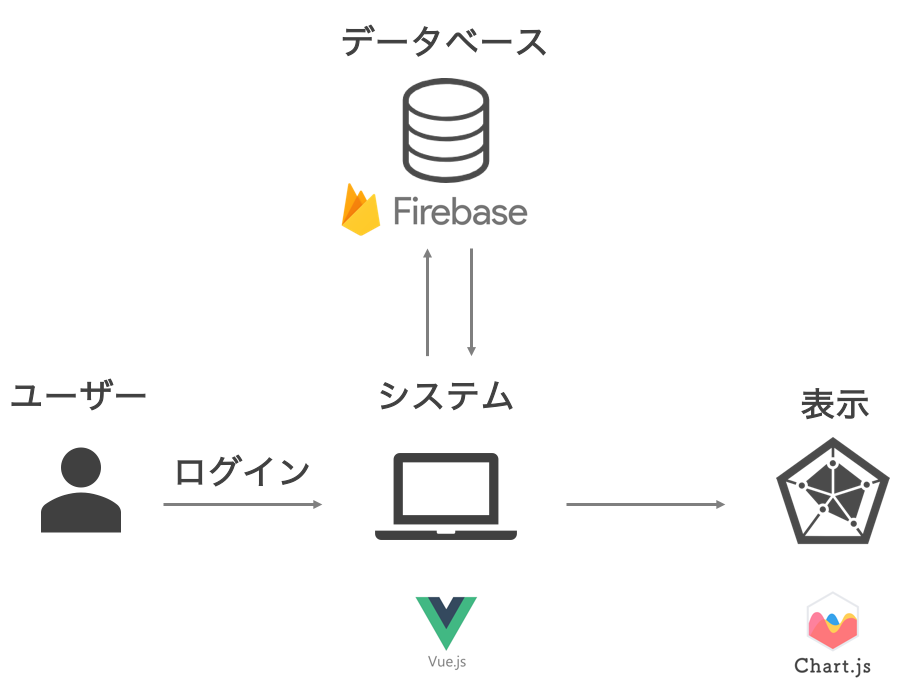
\includegraphics[width=100mm]{figures/sysytemstrucuture.png}
 \caption{システム構造}
 \label{sysytem}
\end{figure}

\ ページを表示するフロントエンド部分をVue.js,データーを取得するなどのバックエンド部分をFirebaseで行う構造になっている.基本的に全てのデータはFirebaseのRealtime Databaseに依存している.Firebaseは高速な非同期通信を行うことができるため,ユーザにデータのやりとりを感じさせない体験を提供することができる.
\ レーダーチャートを表示する部分に関しては,必要なデータをFirebaseから参照し,データをセットした上でグラフを表示させている.データは非同期通信でリアルタイムに値が更新される.


\section{プロトタイプ制作}

グループワークにおいて個人のスキルを平等に分配し,メンバーの情報を可視化するシステムのプロトタイプ制作を行った.
\begin{figure}[h]
 \centering
   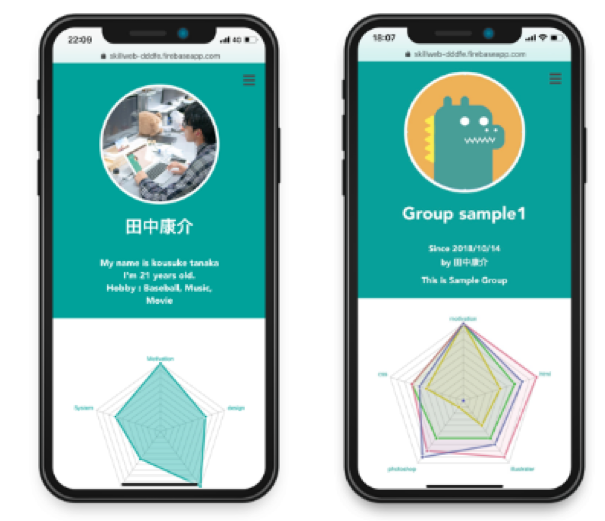
\includegraphics[width=100mm]{figures/gamen.png}
 \caption{プロトタイプの一部}
 \label{gamen}
\end{figure}

\subsection{画面構造}
システムの画面遷移図を図\ref{gamensenni}で表す.システムはディスプレイの大きさに合わせてレイアウトを変えている.
\ ユーザーはログイン画面でログインを行う,ログインの実装にはFirebaseのユーザー認証機能であるFirebase Authenticationを利用している.Firebase Authenticationを用いることで高速でユーザー認証を行うことができる.ユーザー認証はGoogleアカウントを用いて行う.ログインしたのちにユーザーの情報を記載しているホーム画面に遷移する.
\ ホーム画面では自分のスキルを表示したレーダーチャートと基本情報が記載されている.また画面右上のメニューボタンを押すことでメニューが画面右側に表示される.メニューからグループ生成画面,グループ画面,設定画面,テスト画面に遷移することができる.グループ生成画面では次項で説明する.
\ グループ画面では作成されたグループの情報が記載されている.具体的には,所属しているメンバー,メンバー全員のスキルを表示したチャート,チャットが記載されている.所属したメンバーはプロフィール画像で表示しており,プロフィール画像を押すことでメンバーのプロフィール画面に遷移することができる.メンバーのプロフィール画面はホーム画面の構造と同じである.スキルを表示したチャートはメンバー全員のスキルをそのまま表示したチャート,メンバー間の最大値を表示したチャート,メンバー間の平均値を表示したチャートの3種類ある.またチャットはメンバーが投稿したメッセージを非同期で表示することができる.
\ 設定画面ではユーザー自身の情報の登録,変更を行う.またグループ自動生成機能で使用する所属(Occupation)の追加も行う.詳しくはのちに説明する.


\begin{figure}[h]
 \centering
   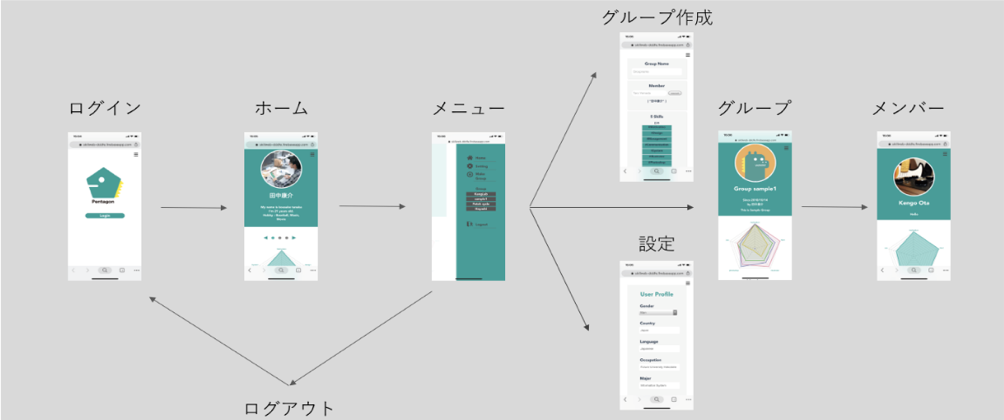
\includegraphics[width=150mm]{figures/gamensenni.png}
 \caption{画面遷移図}
 \label{gamensenni}
\end{figure}

\begin{figure}[h]
 \centering
   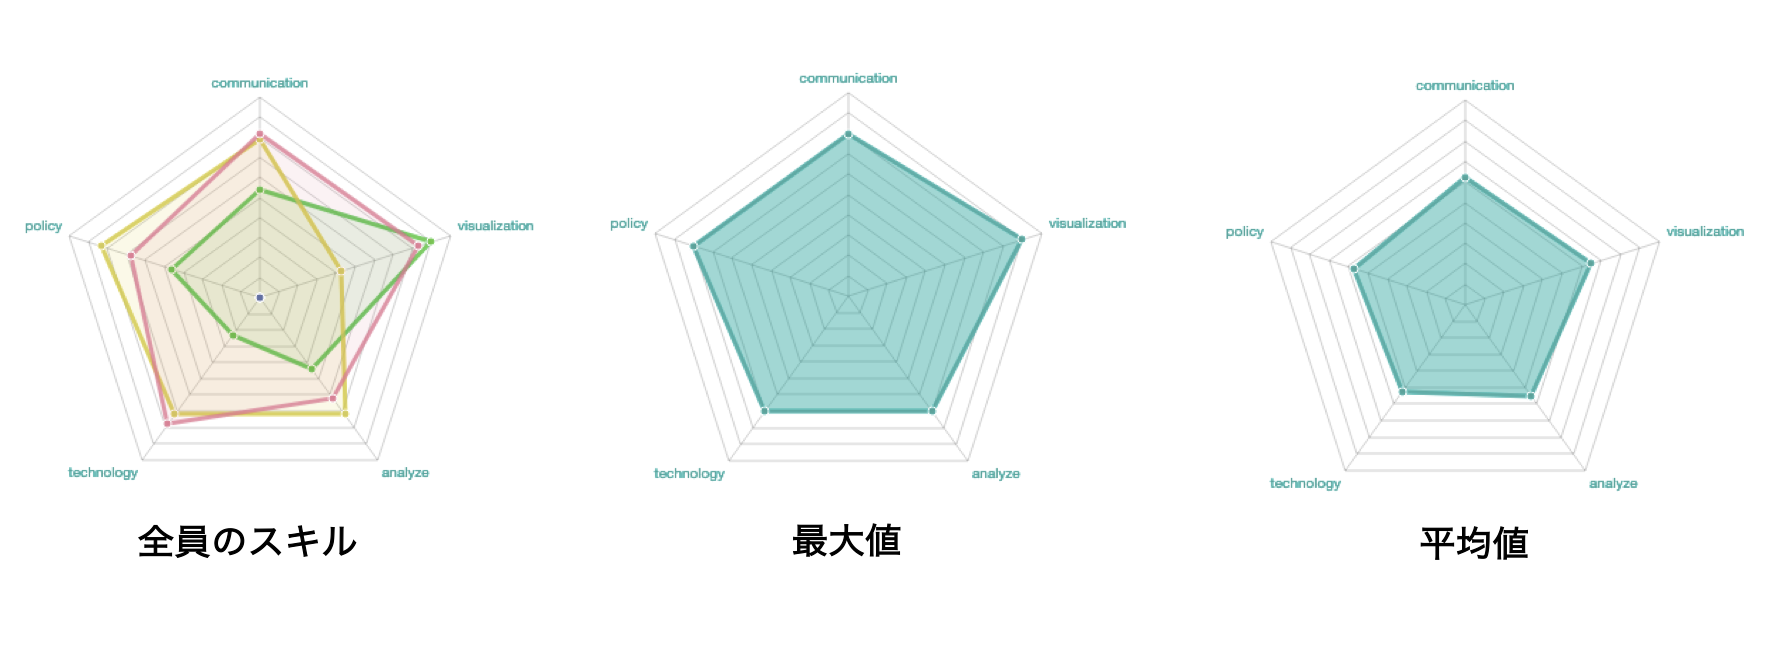
\includegraphics[width=150mm]{figures/chart.png}
 \caption{チャート}
 \label{chart}
\end{figure}


\subsection{グループ自動生成機能}
\subsubsection{グループ生成までの流れ}
グループ自動生成機能の画面は図のようになっている.


\begin{figure}[h]
 \centering
   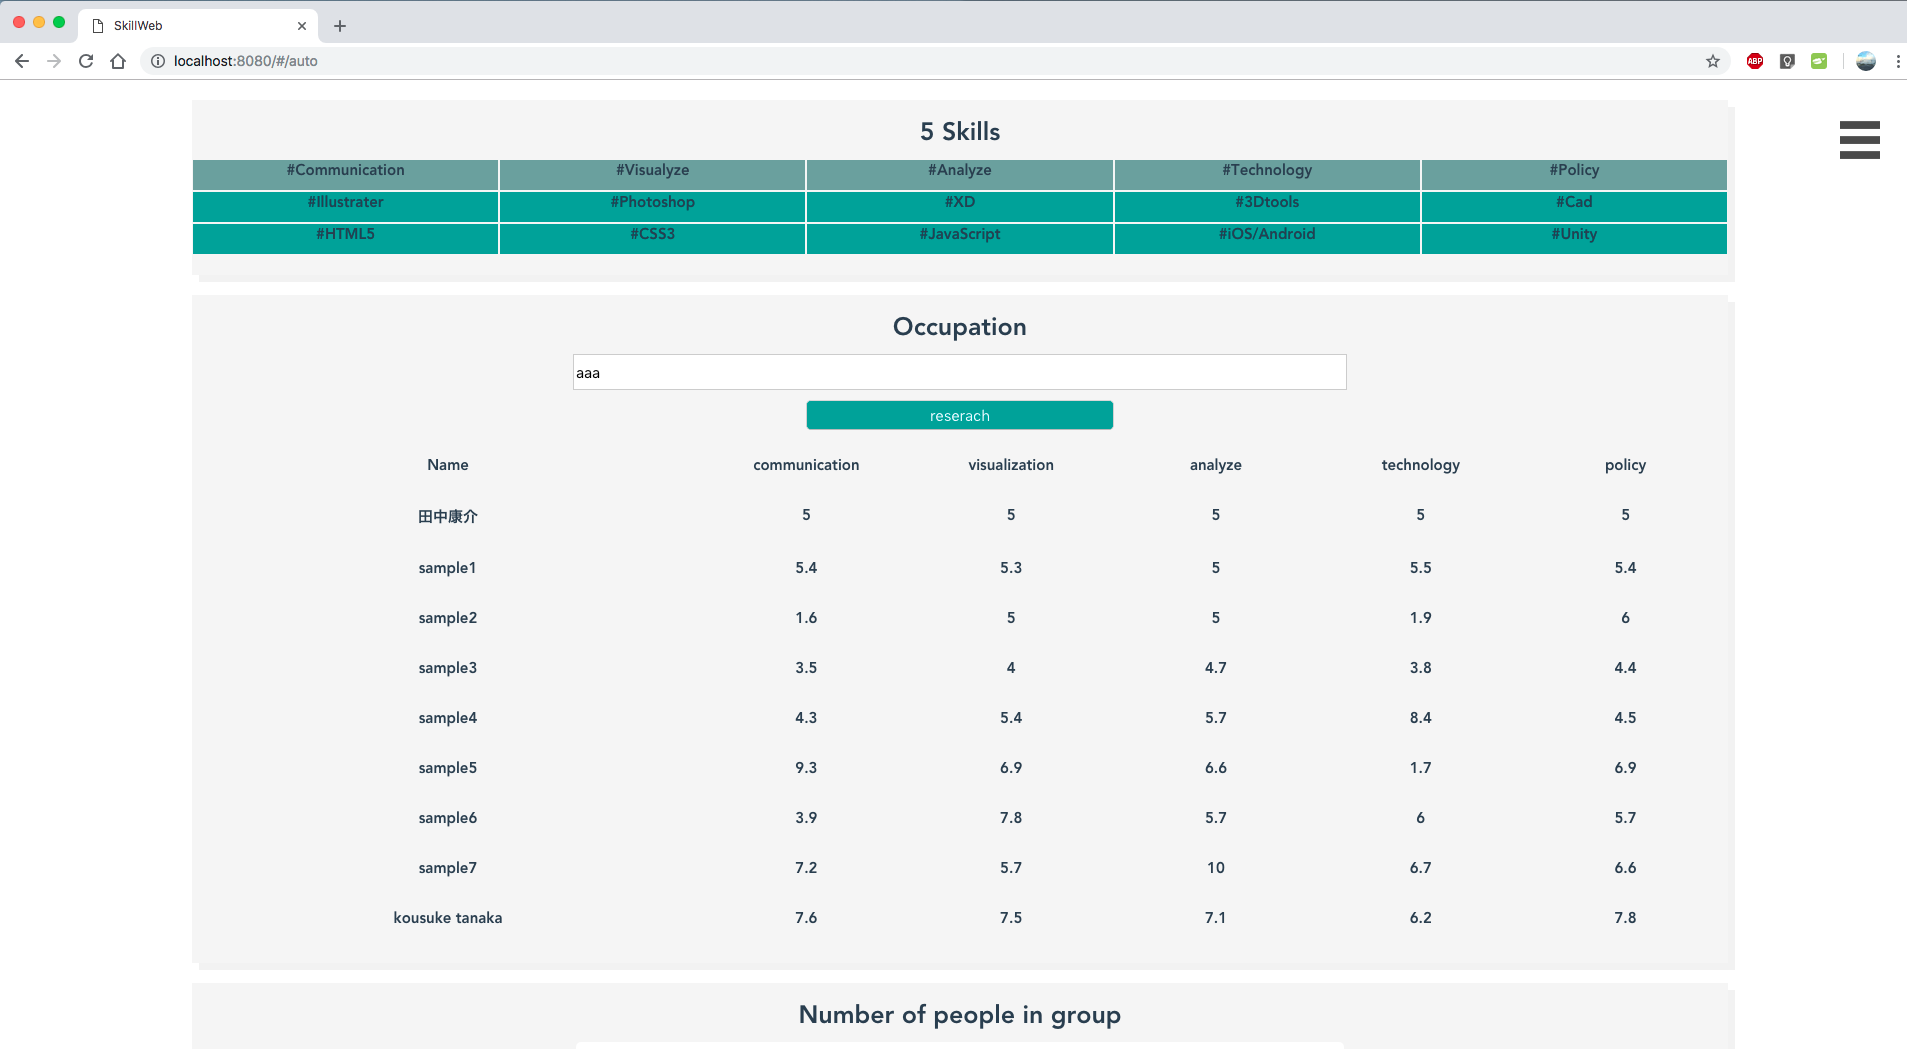
\includegraphics[width=150mm]{figures/groupseisei.png}
 \caption{グループ作成画面}
 \label{groupseisei}
\end{figure}


グループ自動生成までの流れは以下のようになっている.\\
\ 1. 必要な5つのスキルを指定する.\\
\ 2. グループ生成者は所属(Occupation)の検索を行い,検索をした所属に含まれているユーザーを取得する.\\
\ 3. ユーザーと指定したユーザーの5つのスキルが表示される.\\
\ 4. グループメンバーの人数を指定する.\\
\ 5. グループ編成を表示する.\\
\ 6. Firebaseに登録する\\

\subsubsection{グループ自動生成の構造}
グループ自動生成の実装は先行調査を参考に行った\cite{A6}.グループ作成者が指定した5つのスキルの値を以下の式を使用することで個人のスキル総数を出力した.
\begin{equation} 
y_{il} = \sum^{5}_{j=1} x_{il} \\
\end{equation}
$
\  \  \  \  \  \  \  \  \  \  \  \  \  \  \  \  \  \  \  \  \  \   \  \  \  \  \  i : スキル番号 
\  \  \  \  \  \  \  \  \  \  \  \  \  \  \ j : スキル番号 \\
\  \  \  \  \  \  \  \  \  \  \  \  \  \  \  \  \  \  \  \  \  \   \  \  \  \  \ y_{il} : 目的変数
\  \  \  \  \  \  \  \  \  \  \  \  \  \  \ x_{il} : ユーザのスキル値 \\
\  \  \  \  \  \  \  \  \  \  \  \  \  \  \  \  \  \  \  \  \  \   \  \  \  \  \ l : ユーザ番号 \\
$

個人のスキル総数を出力したのちに以下の工程で自動生成を行う.本システムでのグループ自動生成機能はグループ間の能力の差をより均等にするものとした.自動生成の流れは以下である.なお例としてメンバーの総数9人,グループメンバーの人数を3人とする.\\
\ 1. メンバー間のスキル総数を比べ,順に並べる.\\
\ 2. 所属メンバー全員の人数と指定したグループごとの人数からチーム数を割り出す.\\
\ 3. 順に並べているメンバーを図のようにして割り振る.\\
\ 4. 作成した2人組のグループのスキル総数を出力し,グループごとに比べ順に並べる.\\
\ 5. 残りのメンバーをスキル総数が大きな順からグループのスキル総数が小さい方に割り振る.\\
\ 6. グループ編成を出力する.\\
\begin{figure}[h]
 \centering
   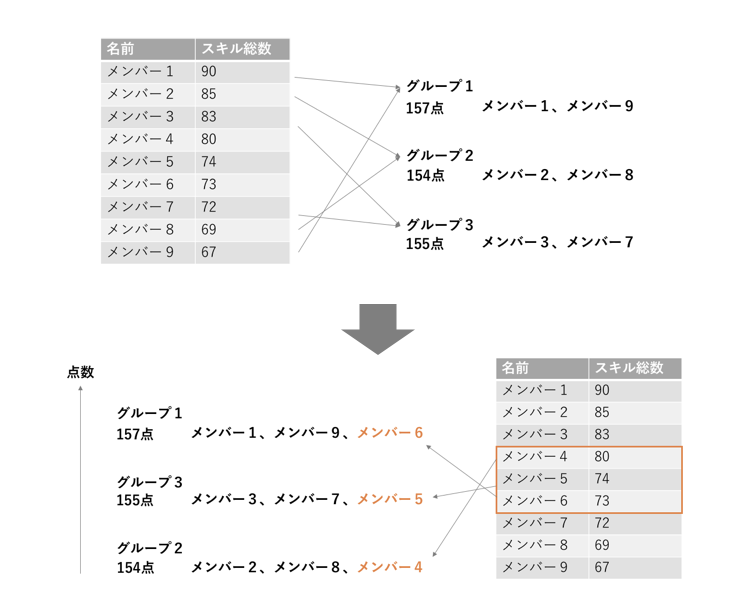
\includegraphics[width=150mm]{figures/auto.png}
 \caption{自動生成機能}
 \label{auto}
\end{figure}





%--------------------------------------------------------------------
\chapter{実験}
本研究で制作したシステムの有用性を判断するために実験を行なった.実験の様子を図で示す.

\begin{figure}[h]
 \centering
   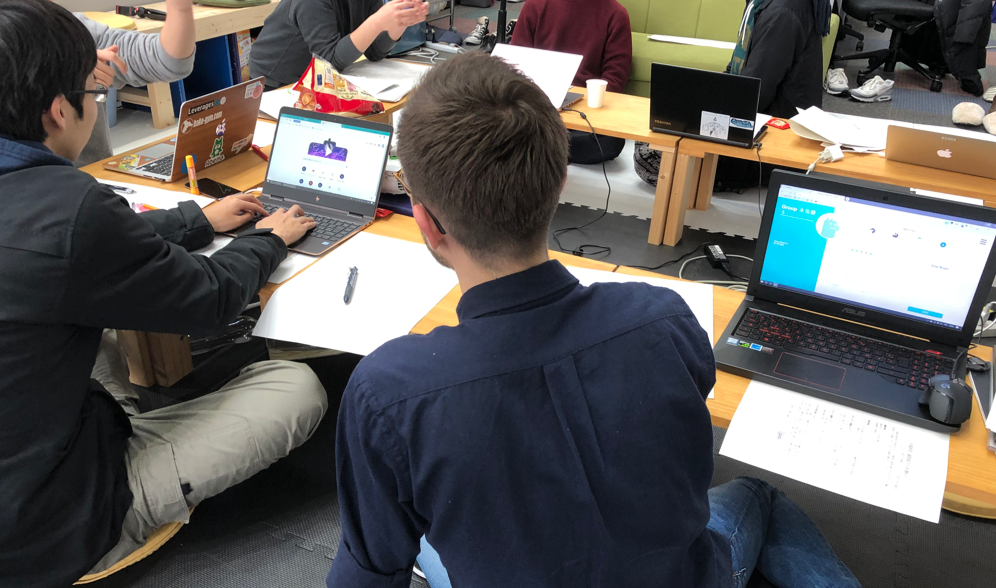
\includegraphics[width=100mm]{figures/zikkennyousu.png}
 \caption{実験の様子}
 \label{auto}
\end{figure}


\section{実験目的}
制作したシステムの新規性はユーザー間のスキルの可視化と共有である。したがって本実験では,「スキルの可視化」に最も着目して行う.またシステムの機能の一つであるグループ自動生成機能の効果を明らかにすることと,システムの改善点を明らかにすることにも着目する.
したがって本実験の目的は,制作したシステムがグループワークの結果にどのように影響を及ぼすかを明らかにし,システムの有用性を判断することとする.
\section{実験方法}
\subsection{実験手順}
本実験は2019年1月18日に行われた.また場所は公立はこだて未来大学をし,被験者は同大学の20歳から22歳の学生18人とした.\\
\ 被験者は3人で1グループを作り,テーマに基づいてグループワークを1人2回行った.1回目と2回目ではグループのメンバー構成を変えた.1回目でシステムを使用するグループ群(A集合)とシステムを使用しないグループ群(B集合)に分け,2回目でその逆を行い,2回グループワークが終わった後にグループワークの満足度についてアンケートに答えてもらった.

\begin{figure}[h]
 \centering
   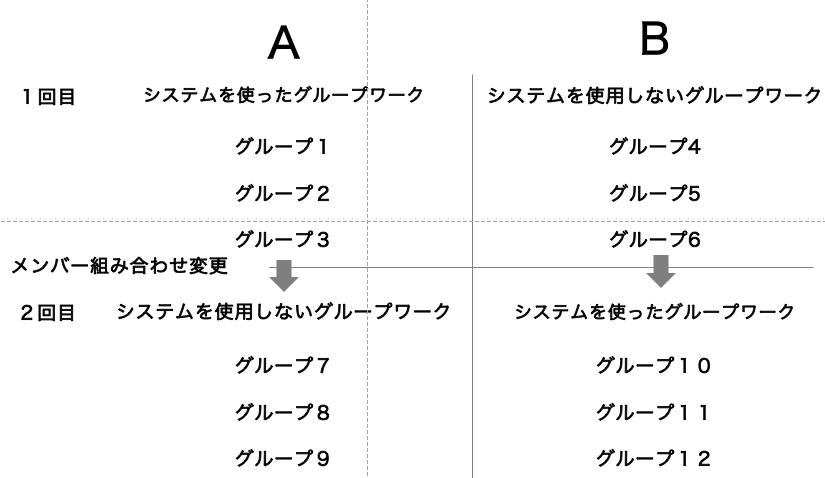
\includegraphics[width=100mm]{figures/zikken1.png}
 \caption{実験詳細}
 \label{zikken1}
\end{figure}

\ A集合とB集合を作成した理由は,システムの有用性を確かめる上で,先にシステムを使用するグループ群と後に使用するグループ群を作ることで条件を平等にする必要があると推測したためである.またシステムを使用するグループには,システムの使用方法を実験を始める前に説明し,必要なデータを登録させ,グループ自動生成機能を用いてメンバーを振り分けた.\\
\ グループワークのテーマをそれぞれ,「文房具とIT」,「おもちゃとIT」とし,テーマに沿って新たなアイデア,プロダクトを提案してもらった.
テーマの決定理由については実験準備で説明する.また制限時間を30分とした.グループワークの最後にグループとしての案を発表してもらい撮影をした.またアイデアについてのスケッチを回収した.

\subsection{評価方法}
評価手法は先行研究\cite{A17}を参考にし,主観的評価と客観的評価の二つを行なった.
\subsubsection{主観的評価}
実験後のアンケートによる主観的評価を行なった.アンケートの質問項目の1問目は,システムを使用したグループと使用していないグループのどちらが上手くいったかを使用したグループ,使用していないグループのどちらかを選択してもらった.2問目は,スキルチャートを見ることで相手への理解が深まったかを,とても深まった,深まった,どちらでもない,深まらなかった,全く深まらなかったの5つから選択してもらった.3問目は,本システムをまた利用したいと思うかを,とてもそう思う,そう思う,どちらでもない,そう思わない,全くそう思わないの5つから選んでもらった.4問目は,システムを利用した感想を自由記述で書いてもらった,5問目は,システムの改善案を自由記述で書いてもらった.\\
\ 質問項目の意図は,システムを使用した場合としてない場合の違い,スキルの可視化がグループワークに与える影響,システムの改善点を調べるの3点であった,                                                         
\subsubsection{客観的評価}
客観的評価はグループワークの最後に行うアイデアの説明とそのスケッチから創造性に関する評価を行なった.先行研究\cite{A18}を参考にし,アイデアをFinkeら\cite{A19}の認知的アプローチによる創造性評価の方法を用いて評価を行なった.上記の方法はデザインの専門家によって,実用性と独創性の二次元として,デザイン成果物に関してそれぞれ1から5までの5段階評価した.本実験でも実用性と独創性の2軸で評価を行い,合計得点を創造性成果物の評価得点とした.

\section{実験準備}
\subsubsection{使用する5つのスキル}
実験のグループワークで使用する5つのスキルは「コミュニケーション」,「ビジュアル化」,「分析能力」,「テクノロジー」,「ポリシー」とした.\\
\ 5つのスキルの選考方法は,相島ら\cite{A5}のDTMPメソッドを参考にした.第3章でも説明したDTMP系統の中のマネジメント能力(Management)は,本実験のグループワークは短期的なものであるため取り入れず,デザイン(Design)を「ビジュアル化」と「分析能力」に分散し,ポリシー(Policy)を「コミュニケーション」と「ポリシー」に分散した.

\subsubsection{グループワークのテーマ決定}
グループワークのテーマを決定する上でグループワークで使用する5つのスキルを使用することを必要条件とした.
5つのスキルのうち,「コミュニケーション」と「ポリシー」はグループワークを遂行する上での能力とし,「ビジュアル化」「分析能力」「テクノロジー」は個人の知識による能力とした.したがってグループワークのテーマは3つの知識を使用できるものからアイデアを複数出し,最終的に2つに絞った.また制限時間が30分であるため,テーマの範囲を一定数狭くした.

\subsubsection{スキル入力ページの作成}
実験を行うにあたって,使用する5つのスキルをアンケートに答えて,スキルに対するユーザーの能力値を出力するページを作成した.アンケート項目を作成するにあたり,各スキルの定義を行なった.\\
\ 「コミュニケーション」は,色々な価値観や背景を持つ人々による集団において,相互理解を深め,共感しながら人間関係やチームワークを形成できるものと定義した.\\
\ 「ビジュアル化」は,複雑な物事をビジュアル化し抽象的にわかりやすく伝えることができる能力と定義した.\\
\ 「分析能力」は,「事実」や「根拠の明確でない推測」などを正確に見極め,さらに,内在している論理や構造などを的確にとらえていける能力,データから問題を解明するプロセスを構想する力とした.\\
\ 「テクノロジー」は,情報技術に関しての知識,関心の度合いと定義した.\\
\ 「ポリシー」は,創造的活動の成果を戦略的に活用でき,創造的プロセスを取り巻く政策を理解できる能力と定義した.\\
\ 定義した後にそのスキルに対する質問項目を1つのスキルに対し5問作成し,アンケートに対する回答データをデータベースに送信するページの実装を行なった.\ref{testtest}.

\begin{figure}[h]
 \centering
   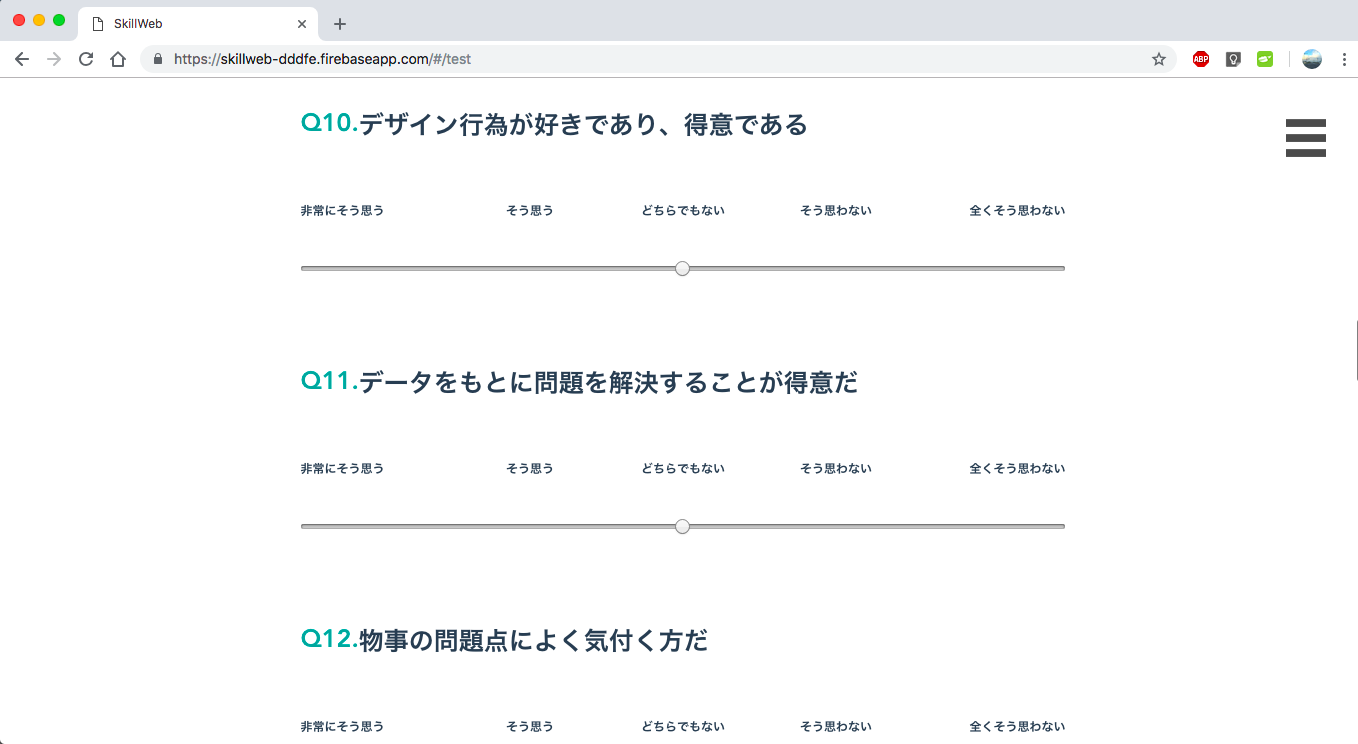
\includegraphics[width=150mm]{figures/test.png}
 \caption{スキル入力ページ}
 \label{testtest}
\end{figure}

\section{実験結果}

\subsection{主観評価}
アンケートによる主観評価結果の結果.システムを使用したグループとシステムを使用していないグループのどちらが上手く進めることができたかという説明に対して,
12名(67\%)がシステムを使用したグループ,6名(33\%)がシステムを使用していないグループと回答した.
\begin{figure}[H]
 \centering
   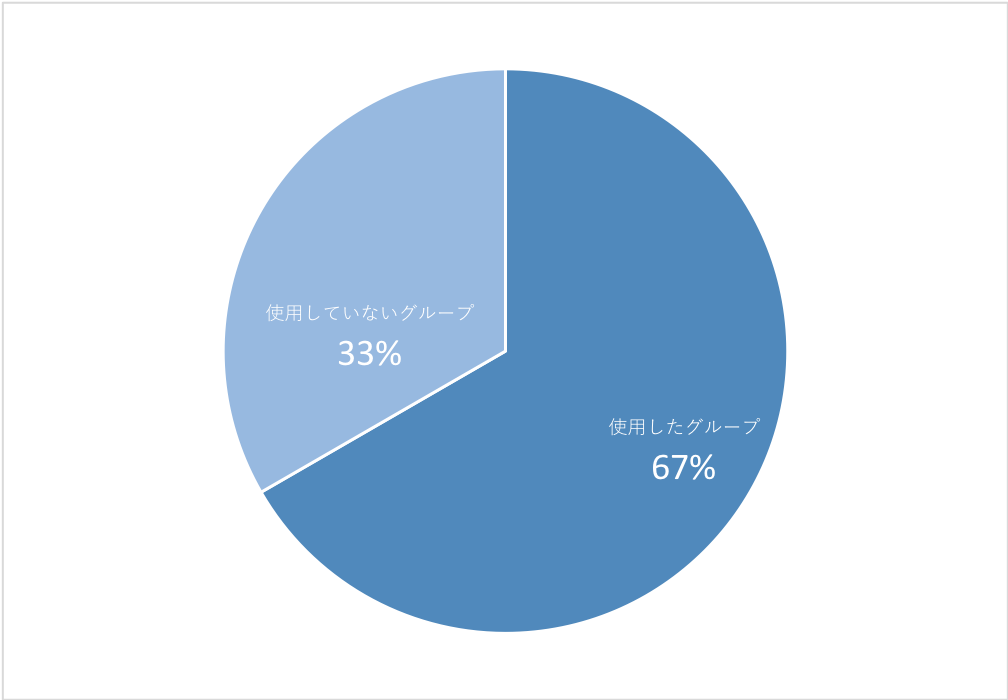
\includegraphics[width=100mm]{honhon0.png}
 \caption{どちらのグループがうまくいったか}
 \label{testtest}
\end{figure}

スキルチャートを見ることで相手への理解が深まったかという質問に対して,3名(17\%)がとても深まった,11名(61\%)が深まった,3名(17\%)がどちらでもない,1名(6\%)が深まらなかった,0名(0\%)が全く深まらなかったと回答した.
\begin{figure}[H]
 \centering
   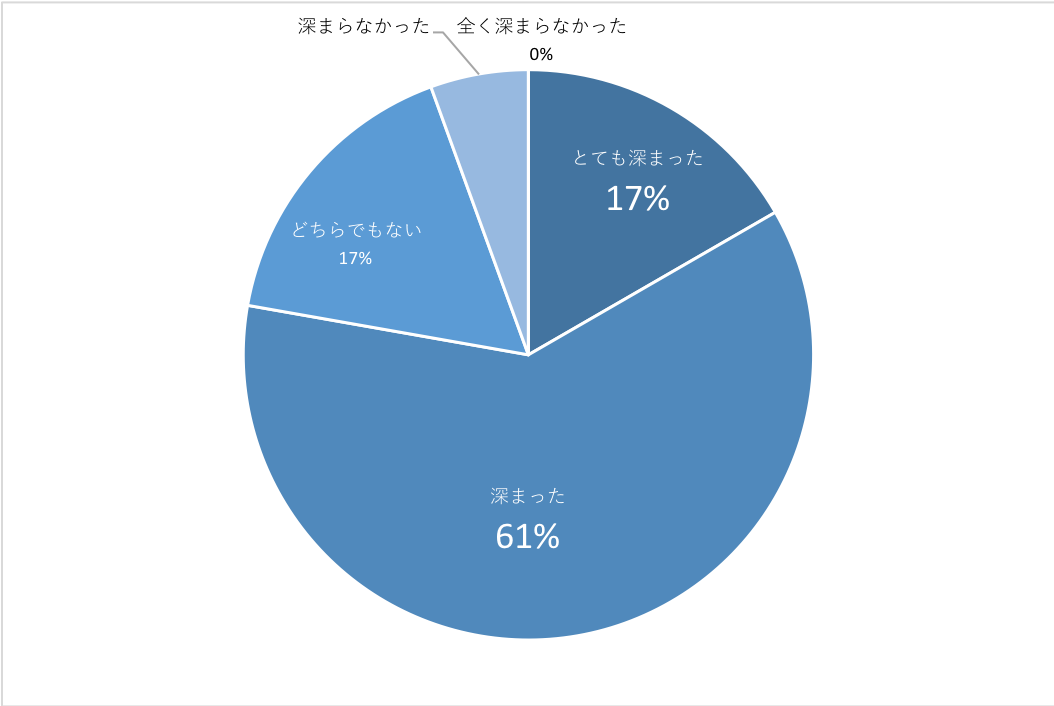
\includegraphics[width=100mm]{honban2.png}
 \caption{チャートを見ることで相手への理解が深まったか}
 \label{testtest}
\end{figure}

本システムをまた利用したいかという質問に対して,4名(22\%)がとてもそう思う,10名(56\%)がそう思う,3名(17\%)がどちらでもない,1名(6\%)がそう思わない,0名が全くそう思わないと回答した.
\begin{figure}[H]
 \centering
   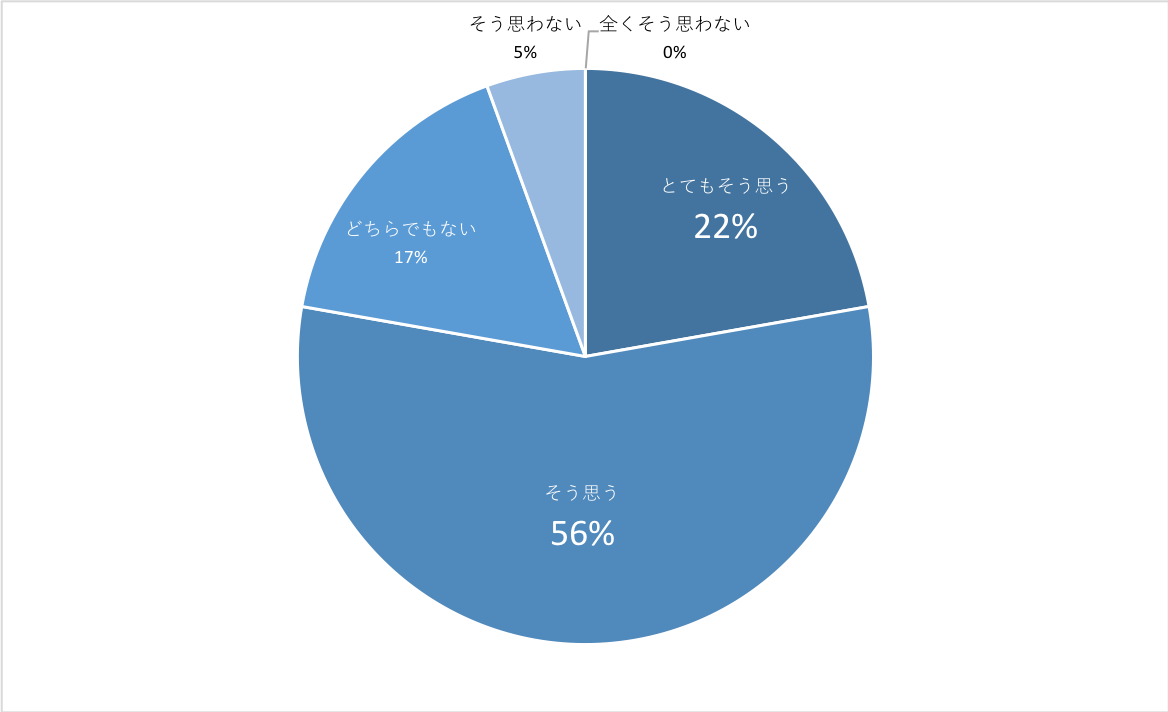
\includegraphics[width=100mm]{honban1.png}
 \caption{本システムをまた利用したいか}
 \label{testtest}
\end{figure}

システムを利用した感想の自由記述欄では,「相手のスキルがわかることで,アイデアから形にする過程がスムーズにいった」という意見や「グループ分けをするのに役に立ちそう」などの意見が得られた.
システムの改善案の自由記述では,「スキルの入力方法が自己申告制なので信憑性が低いのではないか」という意見や「チャートが誰のチャートか見づらかった」などのユーザーインターフェースデザインの意見も得られた.

\subsection{客観的評価}
前述の創造性成果物の評価手法を用いて以下の結果が得られた(表\ref{客観的評価}).表\ref{客観的評価}の「スキル最大値」は,グループ内の5つのスキルの各最大値を足したものを表しており,スキル平均値はメンバー全員の5つのスキルの各平均値を足したものを表している.\\
システムを使用した場合の独創性得点の平均は2.75,分散は0.81,実用性得点の平均は3.83.分散は1.39,総合得点の平均は6.42,分散は1.39,スキル最大値の平均は35.4,分散は14.1,スキル平均値の平均は28.7,分散は6.84であった.\\
システムを使用していない場合の独創性得点の平均は3.58,分散0.62,実用性得点の平均は4.08.分散は1.04,総合得点の平均は7.67,分散は2.35,スキル最大値の平均は35,分散は13.6,スキル平均値の平均は28.6,分散は8.37であった.\\

\ 
\begin{table}[H]
\begin{center}
  \begin{tabular}{cccccc} \hline
  システム使用\tabularnewline \hline
  グループ名&独創性&実用性&創造性得点
  &スキル最大値 & スキル平均値\tabularnewline \hline
    グループ1&3&3&6&29.1 &25.4\tabularnewline
    グループ2&3&4&7& 31.5&25.3 \tabularnewline
    グループ3&2&4&6 &37.8&29.3\tabularnewline
    グループ10&4.5&4.5&9&37&28.5 \tabularnewline
    グループ11&2&4&6&39.7&31.4 \tabularnewline
    グループ12&2&3.5&5.5&37.1&32 \tabularnewline \hline 
     &平均2.75&平均3.83&平均6.42&平均35.4&平均28.7\tabularnewline
    &分散0.81&分散0.22&分散1.39&分散14.1&分散6.84\tabularnewline 
      \hline \hline 
   システム不使用\tabularnewline \hline 
    グループ4&3&5&8&31.2&25.6 \tabularnewline
    グループ5&4&4&8&28.6&24.9 \tabularnewline
    グループ6&4.5&4.5&9 &36.9&28.3\tabularnewline
    グループ7&2.5&4&6.5&37.2&29.6 \tabularnewline
    グループ8&3&2&5 &38.4&29.8\tabularnewline
    グループ9&4.5&5&9.5&37.5&33.6 \tabularnewline
         \hline
         &平均3.58&平均4.08&平均7.67&平均35&平均28.6\tabularnewline 
    &分散0.62&分散1.04&分散2.35&分散13.6&分散8.37\tabularnewline \hline
  \end{tabular}
  \caption{客観的評価}
  \label{客観的評価}
  \end{center}
\end{table}

\section{考察}
実験を行なった結果,主観的による評価で67\%の被験者が「システムを使用したチームの方がグループワークが上手くいった」と回答していることから,過半数
の被験者がシステムを使用した方が満足のいくものだったと感じているのに対し,客観的による創造性成果物の評価ではシステムを使用したグループの方が成果物の評価が低いことがわかった.しかし,システムを使用していないグループ群の成果物の評価の分散が,システムを使用しているグループ群の成果物の評価の分散より高いことから,システムを使用したグループが創造性に関して,より良い結果を出すとは考えにくいが,システムのグループ自動生成機能が「成果の安定」をもたらすという観点では有用であることが示唆された.\\
\ スキルの可視化をすることによって78\%が相手への理解が「深まった」,もしくは「とても深まった」と回答していることと、スキルのチャートがあることによってチーム内の役割分担をすることができたという意見が多数あったことから,チーム内の役割分担,効率性の観点では有用性が高いことが示唆される.\\
\ 以上のことからシステムを使用することで,チーム間の差はなくなるが,創造性の成果物に関しての点数は低くなるため,第2章で定義した成果目的グループワークでは有用性は少なくいと考えられる.そこで学習者の学習程度を評価基準とし,学習課題に対する共通の関心や問題をメンバー構成の主体とする,学習目的グループワークでの使用が推奨すると考えられる. そこで本実験で行われた成果目的型グループワークではなく,学習目的型グループワークでの実験が必要であることを示唆した.


%--------------------------------------------------------------------
\chapter{結論と今後の展開}
\section{まとめ}
本研究では,グループワークと創造性に着目し,スキルの可視化とグループの自動生成を行うことでグループワーク
を支援するシステムの提案を行った.\\
\ グループワークと創造性に着目したシステムを制作する上で,グループワークの現状を把握するためにアンケート調査を行い,自分の視野が広がる,成長できるなどの理由から自分と異なるスキルを持った人とグループワークを行いと思っている人が過半数であることを明らかにした.
\ そこでグループ内のスキルを可視化し、共有するシステムの制作を行った.\\
\ システムの有用性を確かめる実験を行なった結果,創造性の向上という観点ではシステムの有用性があるとは考えにくいことが示唆された.しかし成果物の安定やチーム内の役割分担,効率性という観点では,有用性が高いことが判断された.そこで本システムの使用用途は成果目的でのグループワークではなく,学習目的のグループワークで優位な結果が得られる可能性を示唆した.

\section{今後の方針}
本実験では1つのグループワークに対して,30分と短い時間での実験であった.
そのため短いグループワークでのアイデアと
今後の展望として,本研究で行われた成果目的型グループワークの実験ではなく,学習目的型グループワークでの実験が求められる.
学習目的型グループワークでは,学習者の学習の程度を評価基準に行われるため,創造成果物を作成する授業形式での実験が求められる.
まため,より長期的な調査を行うことが示唆される.
また実験のアンケートで得たシステムの改善案では,客観的なスキルのデータでないためデータの信憑性がないことと,ユーザーインターフェースデザインの
ことについて多く見られた.システムを改善していく.





%--------------------------------------------------------------------
\chapter*{謝辞}

Yeahみんなありがとう

%--------------------------------------------------------------------
% 参考文献
\begin{thebibliography}{9}
 \bibitem {A1} 上平崇仁:協調的デザイン学習における人間中心設計プロセスの適用, 専修大学情報科学研究所所報, 2011
\bibitem {A2}石井成郎, 三輪和久:創造活動における心的操作と外敵操作のインタラクション, 認知科学, Vol.10, No.4, pp.469-485, 2003.
\bibitem {A3}Kang,N : Proposal and Evaluation of Design
Support Tools for Logical Collaborative Design Process, Archives of design research 2015, vol28, No.4, pp.63-75, 2015.
\bibitem {A4}亀田達也 : 合議の知を求めて—グループの意志決定,共立出版,1997.

\bibitem {A12}創造性学会:http://www.japancreativity.jp/

\bibitem {A13}近藤健次・永井由佳里:創造的になるための変容プロセス:mini-cに着目して,プロジェクトマネジメント学会研究発表大会予稿集 2013.Autumn(0), pp.115-120, 2013

\bibitem {A14}川喜田二郎:創造と伝統-人間の深奥と民主手記の根元を探る,祥伝社, 1993

\bibitem {A15}阿濱志保里:創造性を重視した著作権学習に対応する能力を育成する教育デザイン,山口県立大学学術情報 第11号, pp.93-99, 2018
\bibitem {A10}村谷理沙,阪田真己子:創造性課題における協働性の効果について,情報処理学会第80回大会,pp4-299 - 4-300,2018

\bibitem {A11}西本光志・正田悠・阪田真己子・鈴木紀子:共同創作活動におけるコミュニケーション行動 - 性別による比較 - ,『信学技報』114(189), pp.47-50, 2014

\bibitem {A5}相島雅樹, 塚原康仁, 植木淳郎, 杉浦一徳:DTMPメソッドを用いたグループ編成システムの提案, 研究報告情報システムと社会環境, Vol.2011-IS-115, No.2, pp.1-8, 2011.

\bibitem {A6}橋本弘明, 桑原徹, 秋玉梅, 石川達也, 山下公太郎, 古宮誠一:ソフトウェア開発グループ演習のためのチーム編成の最適化支援, メディア教育研究, Vol.3, No.2, pp.61-69, 2007. 

\bibitem {A7}井上久祥,埴生加奈子:学習者の思考特性に着目したグループ形成支援の方法—協調作業を有効にするグループ形成支援システムのための基礎的研究—,情報処理学会研究報告,2004-GN-53,pp.19-24,2004

\bibitem {A8}小林恵智:プロジェクトリーダーのための [入門] チームマネジメント,PHP研究所,2001

\bibitem {A9}北村清一:FFS理論を活用した成果を生み出すチーム編成と実践的な作業割り振りの提案,プロジェクトマネジメント学会研究発表大会予稿集 2013.Autumn(0), pp.115-120, 2013

\bibitem {A16}Vue.js:https://jp.vuejs.org

\bibitem {A17}高木亜有子,森崎巧一,竹内晴彦:デザイン教育のグループワーク企画・制作における印象評価の活用と制作プロセスの分析,湘北紀要第37号,pp. 17-28,2016

\bibitem {A18}永井由佳里,田浦俊春,原川純一:創造的デザインプロセスをもたらす思考の広がり方の分析方法論の思考 ーデザインプロセスにおける主観的関連の役割,デザイン学研究 BULLETIN OF JSSD,vol. 54,pp. 39-46,2007

\bibitem {A19}Finke,R.A .,Ward ,T .B .and Smith,S.M .:Creative Cognition , Theory ,Research ,and
Applications,A BradfordBook , The MIT Press,
Cambridge,1992 (小橋康章訳,創造的認知 ,森 北 出
版 ,1999 )






\end{thebibliography}


% 以降,付録(付属資料)であることを示す
\appendix

%--------------------------------------------------------------------
\chapter*{付録その1} % \chapter{}を使うと「付録A ***」となる

付録その1(プログラムのソースリストなど)を必要があれば載せる

%--------------------------------------------------------------------
\chapter*{付録その2}

評価実験で得られたグループごとのスケッチを付録その2でまとめる
\begin{figure}[H]
 \begin{minipage}{0.47\hsize}
 \begin{center}
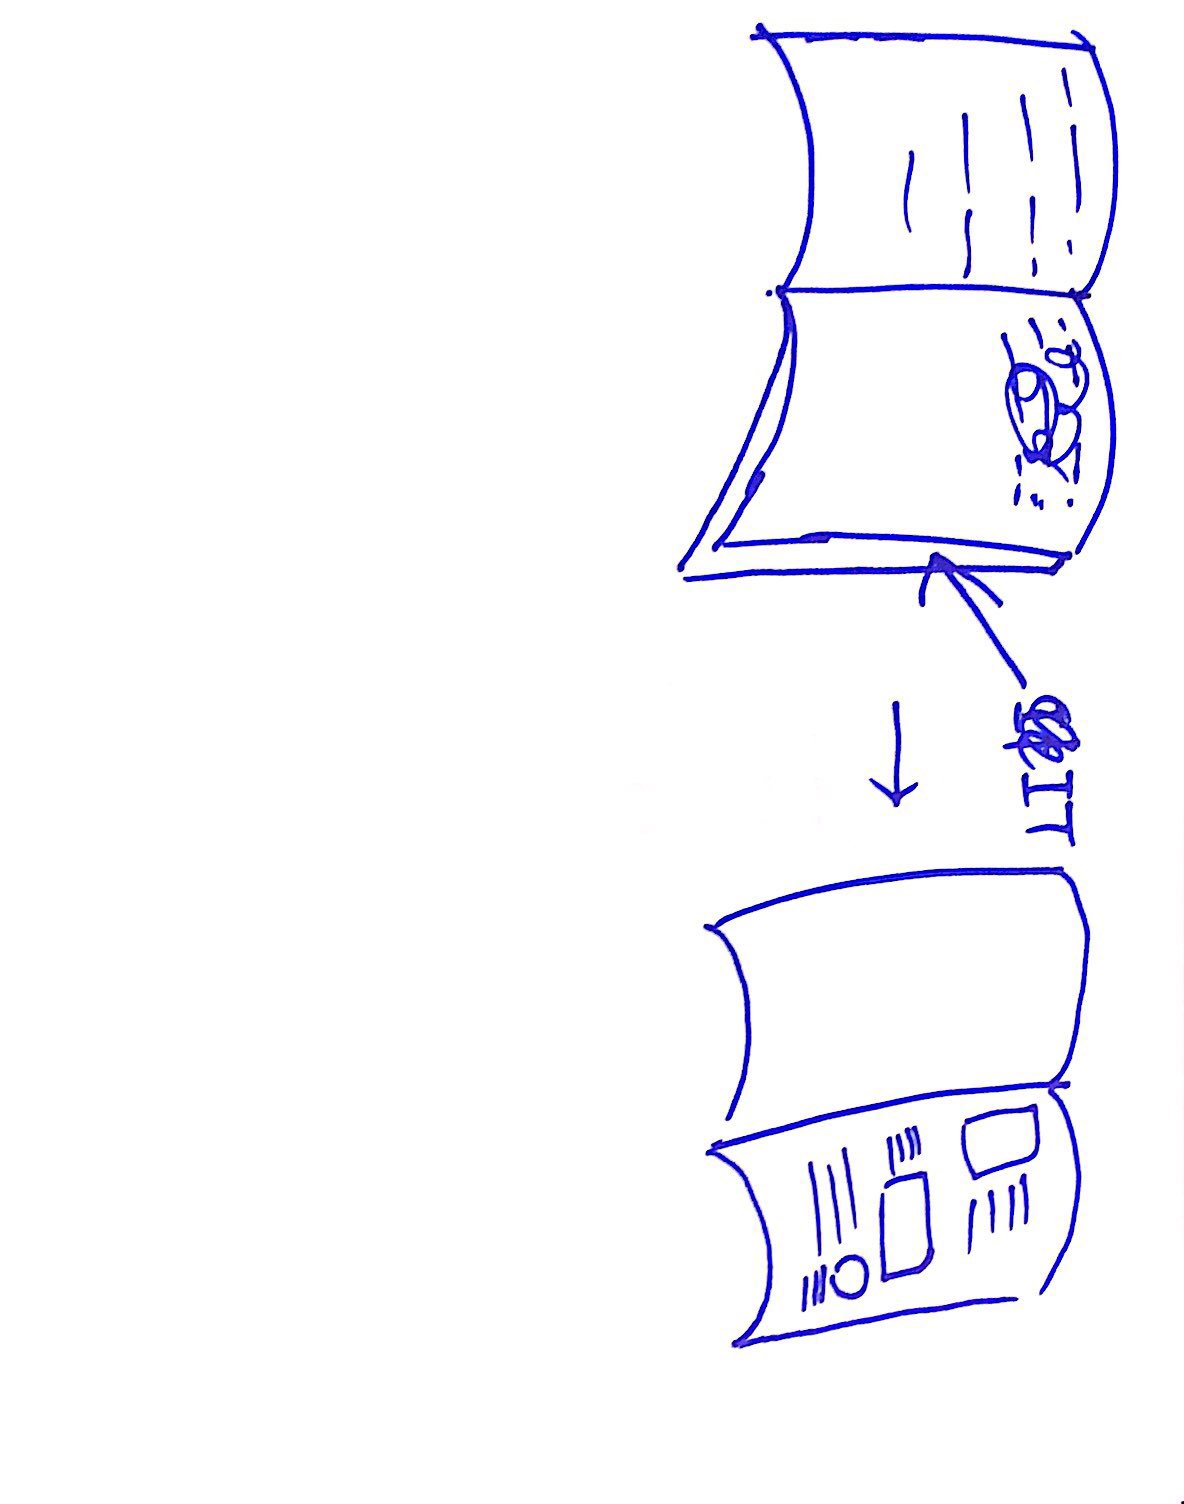
\includegraphics[width=50mm]{figures/group1.jpg}
 \end{center}
 \label{fig:seven}
 \end{minipage}
 \begin{minipage}{0.47\hsize}
 \begin{center}
 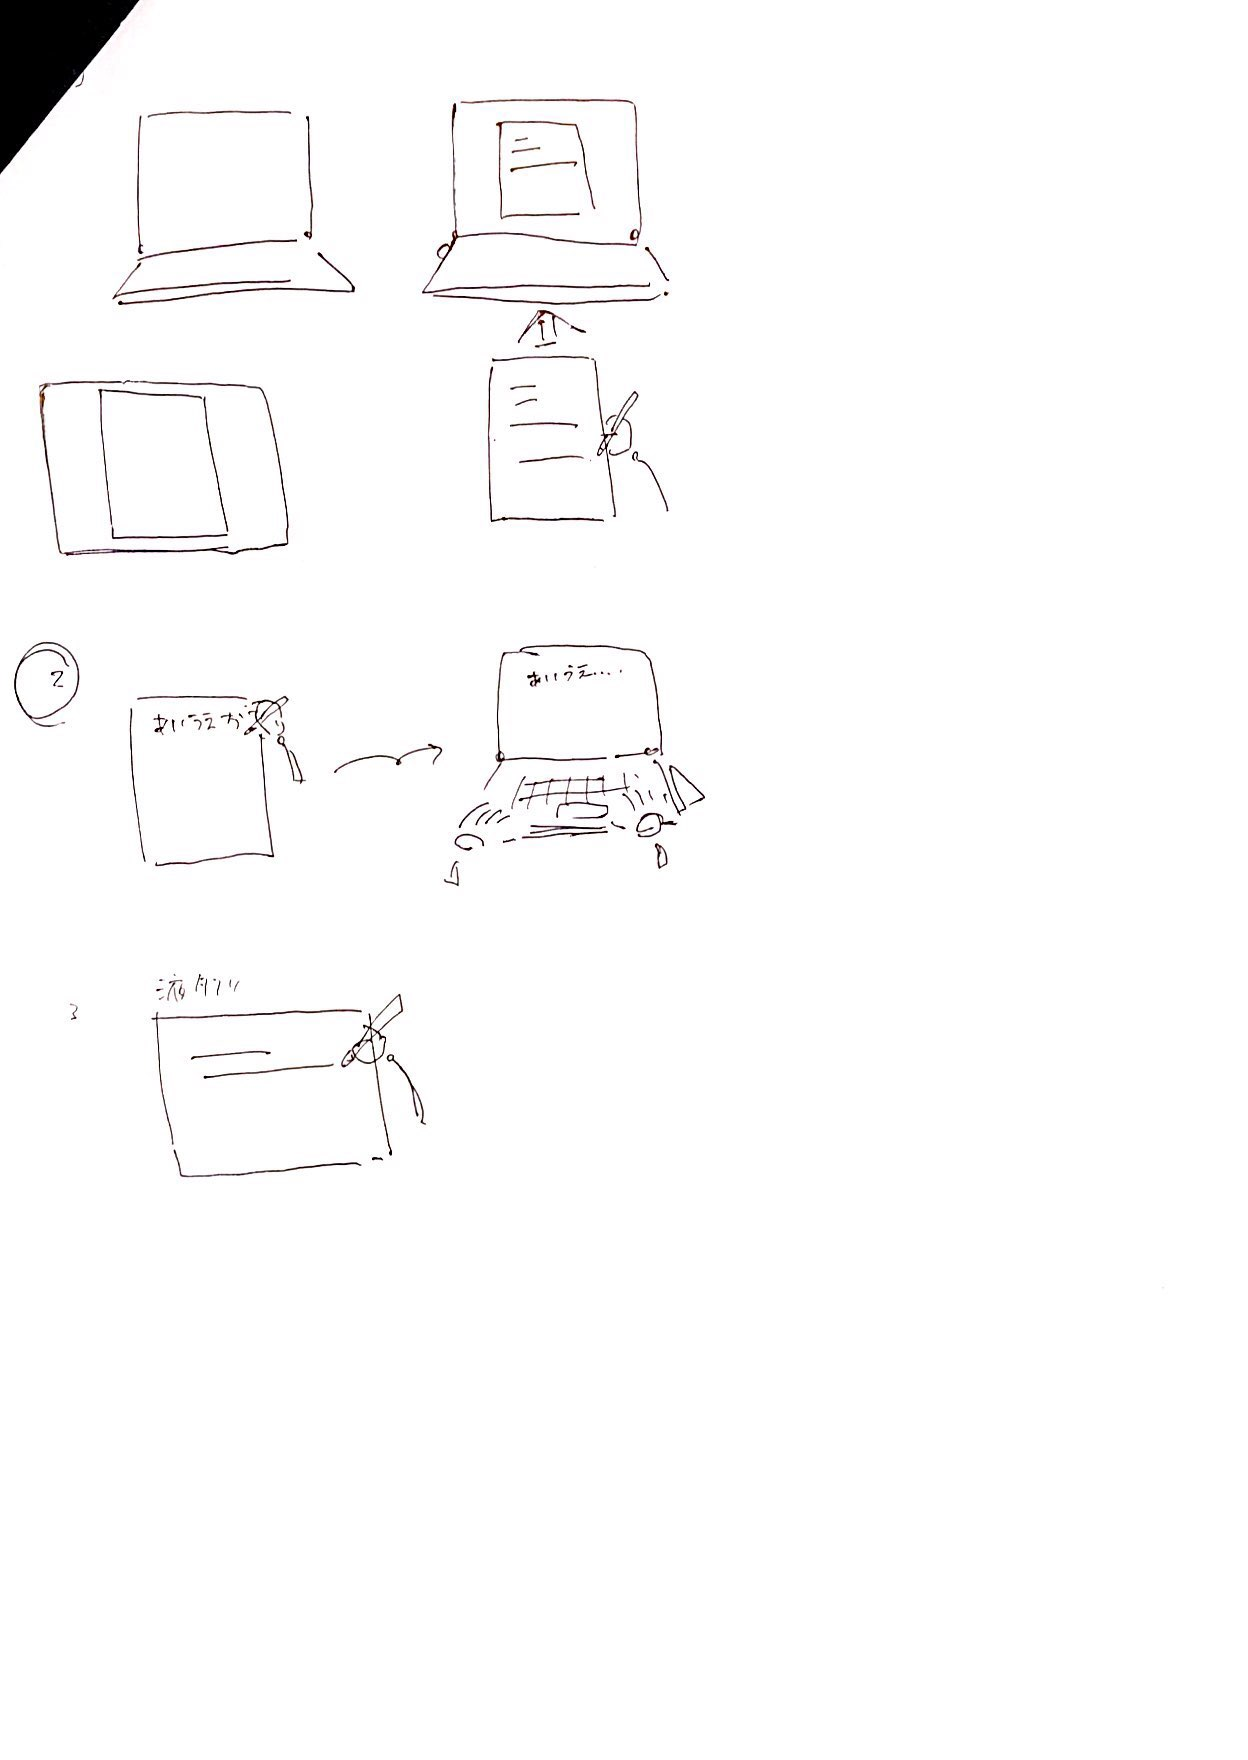
\includegraphics[width=50mm]{figures/group2.jpg}
 \end{center}
 \label{fig:eight}
 \end{minipage}
\end{figure}
\begin{figure}[H]
 \begin{minipage}{0.47\hsize}
 \begin{center}
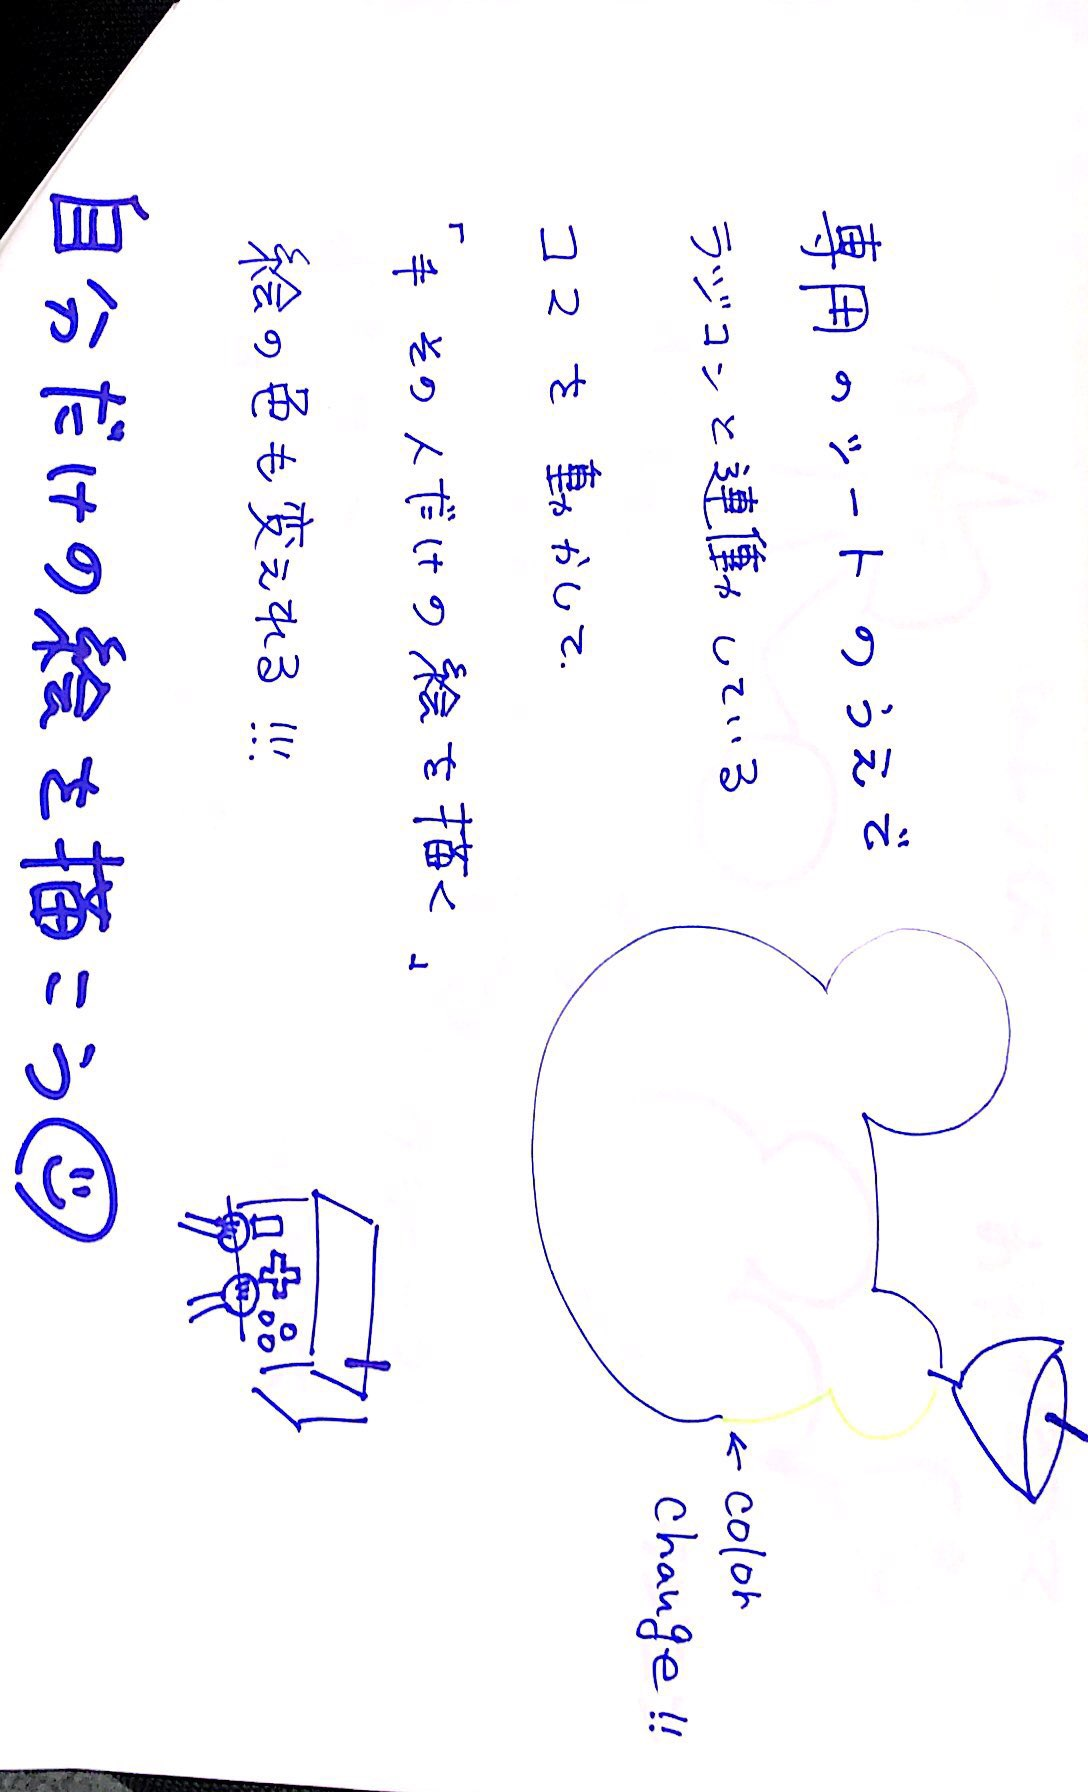
\includegraphics[width=50mm]{figures/group3.jpg}
 \end{center}
 \label{fig:seven}
 \end{minipage}
 \begin{minipage}{0.47\hsize}
 \begin{center}
 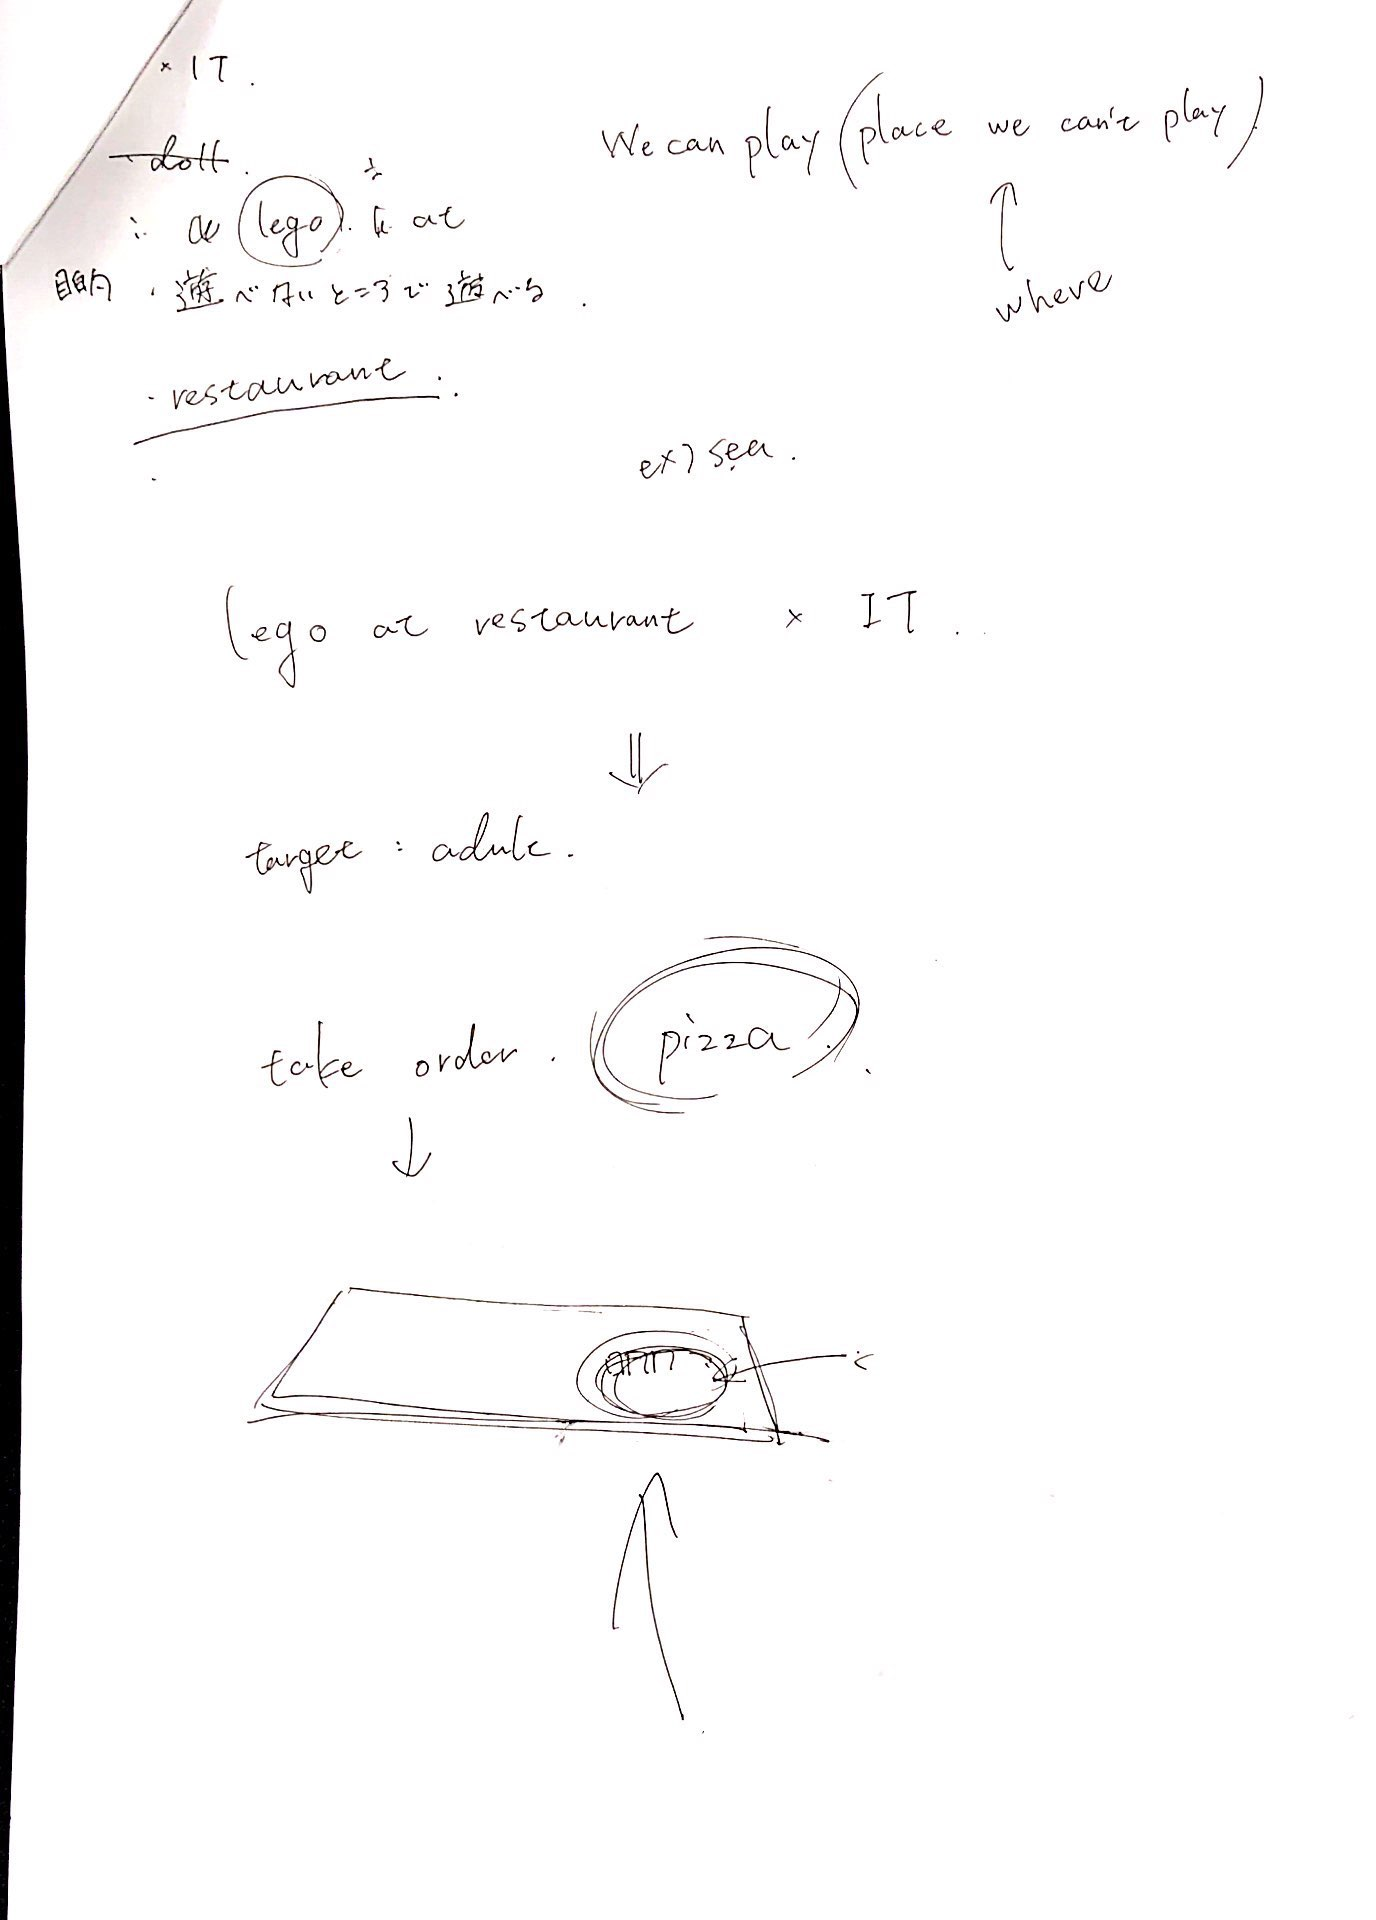
\includegraphics[width=50mm]{figures/group4.jpg}
 \end{center}
 \label{fig:eight}
 \end{minipage}
\end{figure}
\begin{figure}[H]
 \begin{minipage}{0.47\hsize}
 \begin{center}
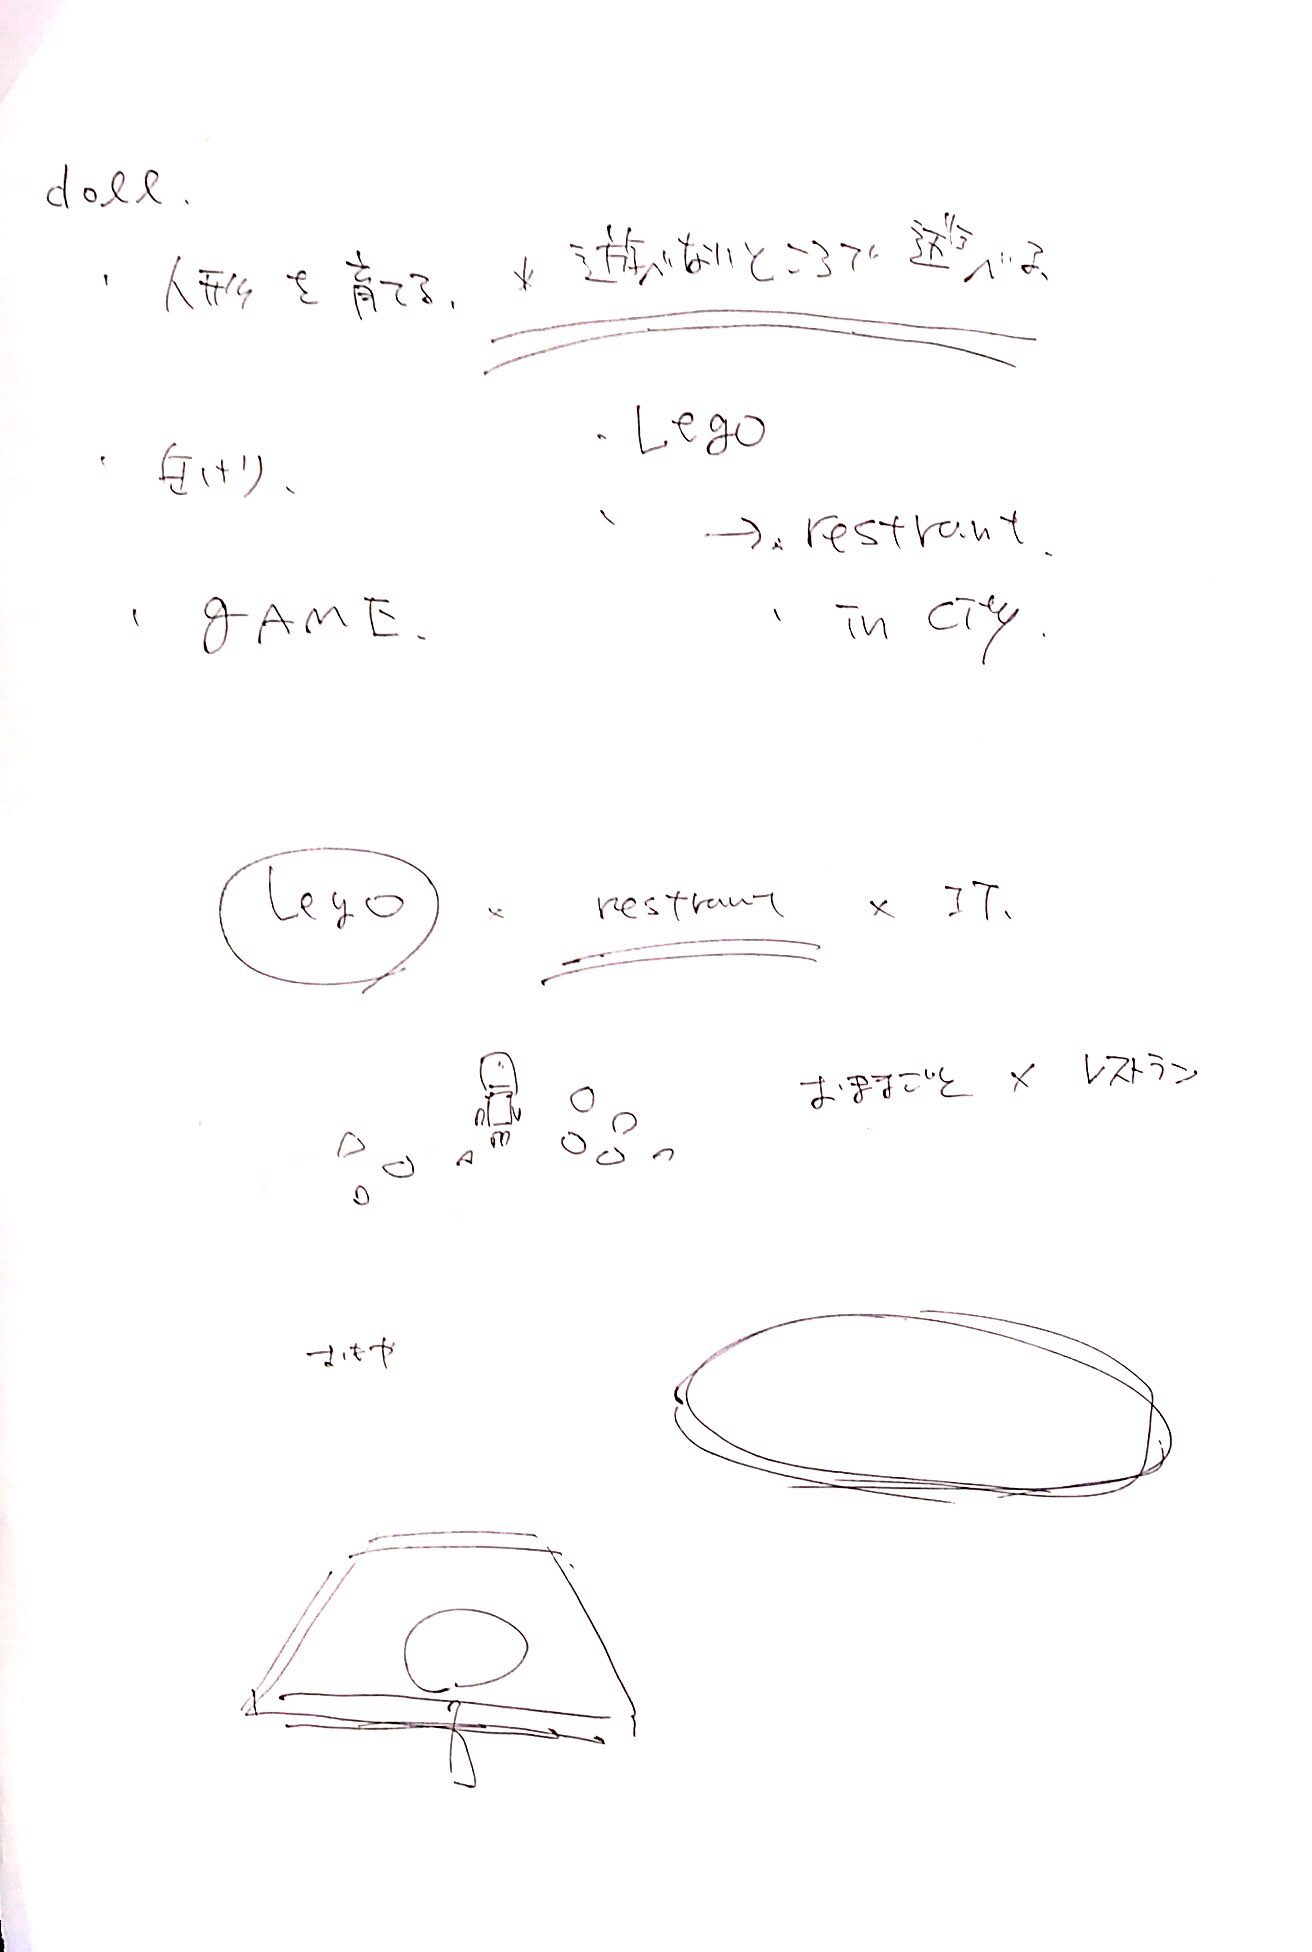
\includegraphics[width=50mm]{figures/group5.jpg}
 \end{center}
 \label{fig:seven}
 \end{minipage}
 \begin{minipage}{0.47\hsize}
 \begin{center}
 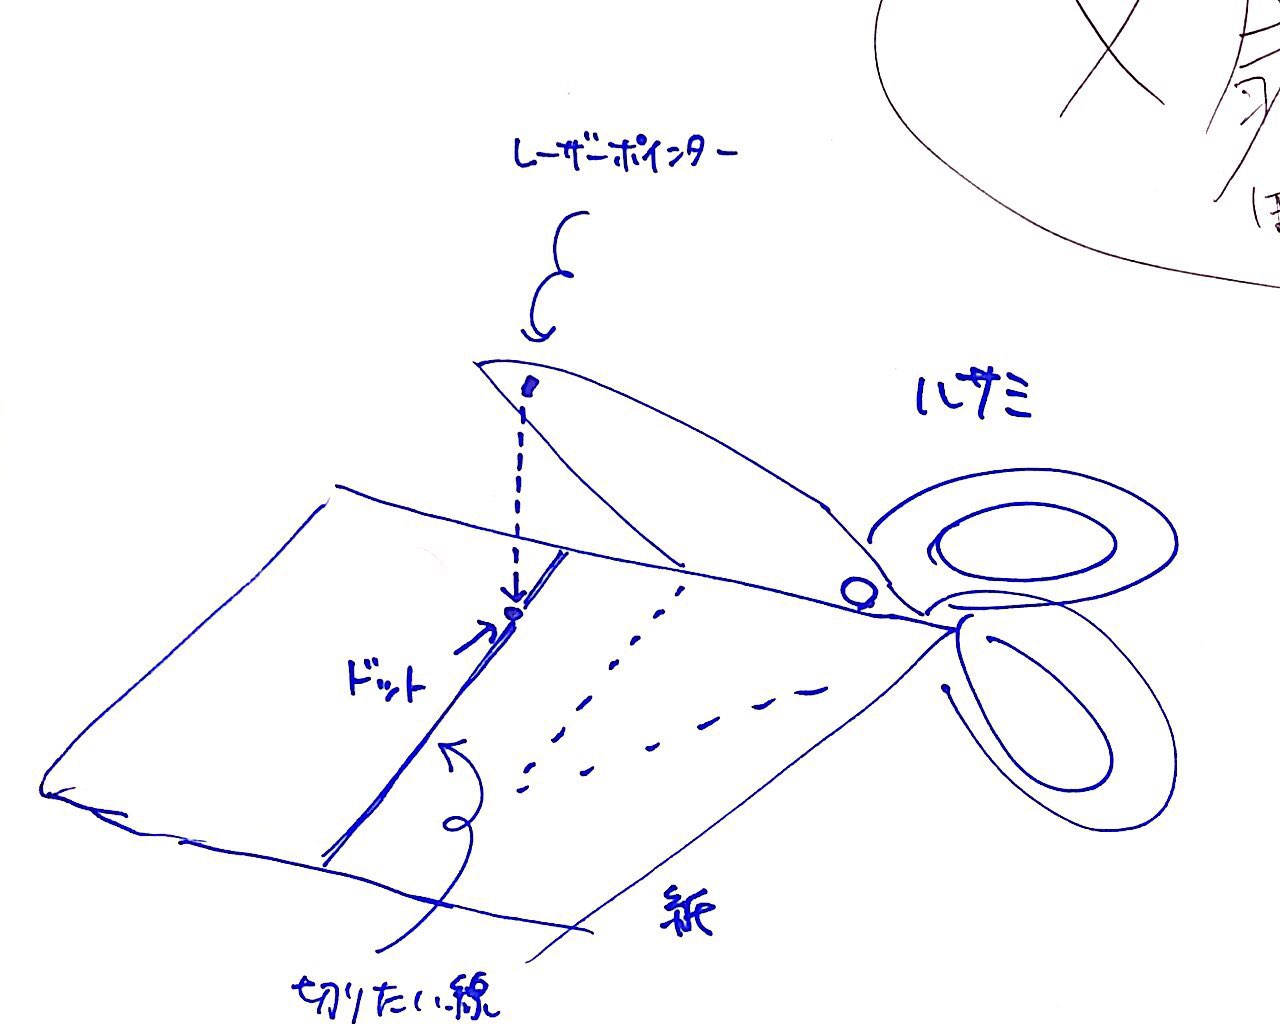
\includegraphics[width=50mm]{figures/group6.jpg}
 \end{center}
 \label{fig:eight}
 \end{minipage}
\end{figure}
\begin{figure}[H]
 \begin{minipage}{0.47\hsize}
 \begin{center}
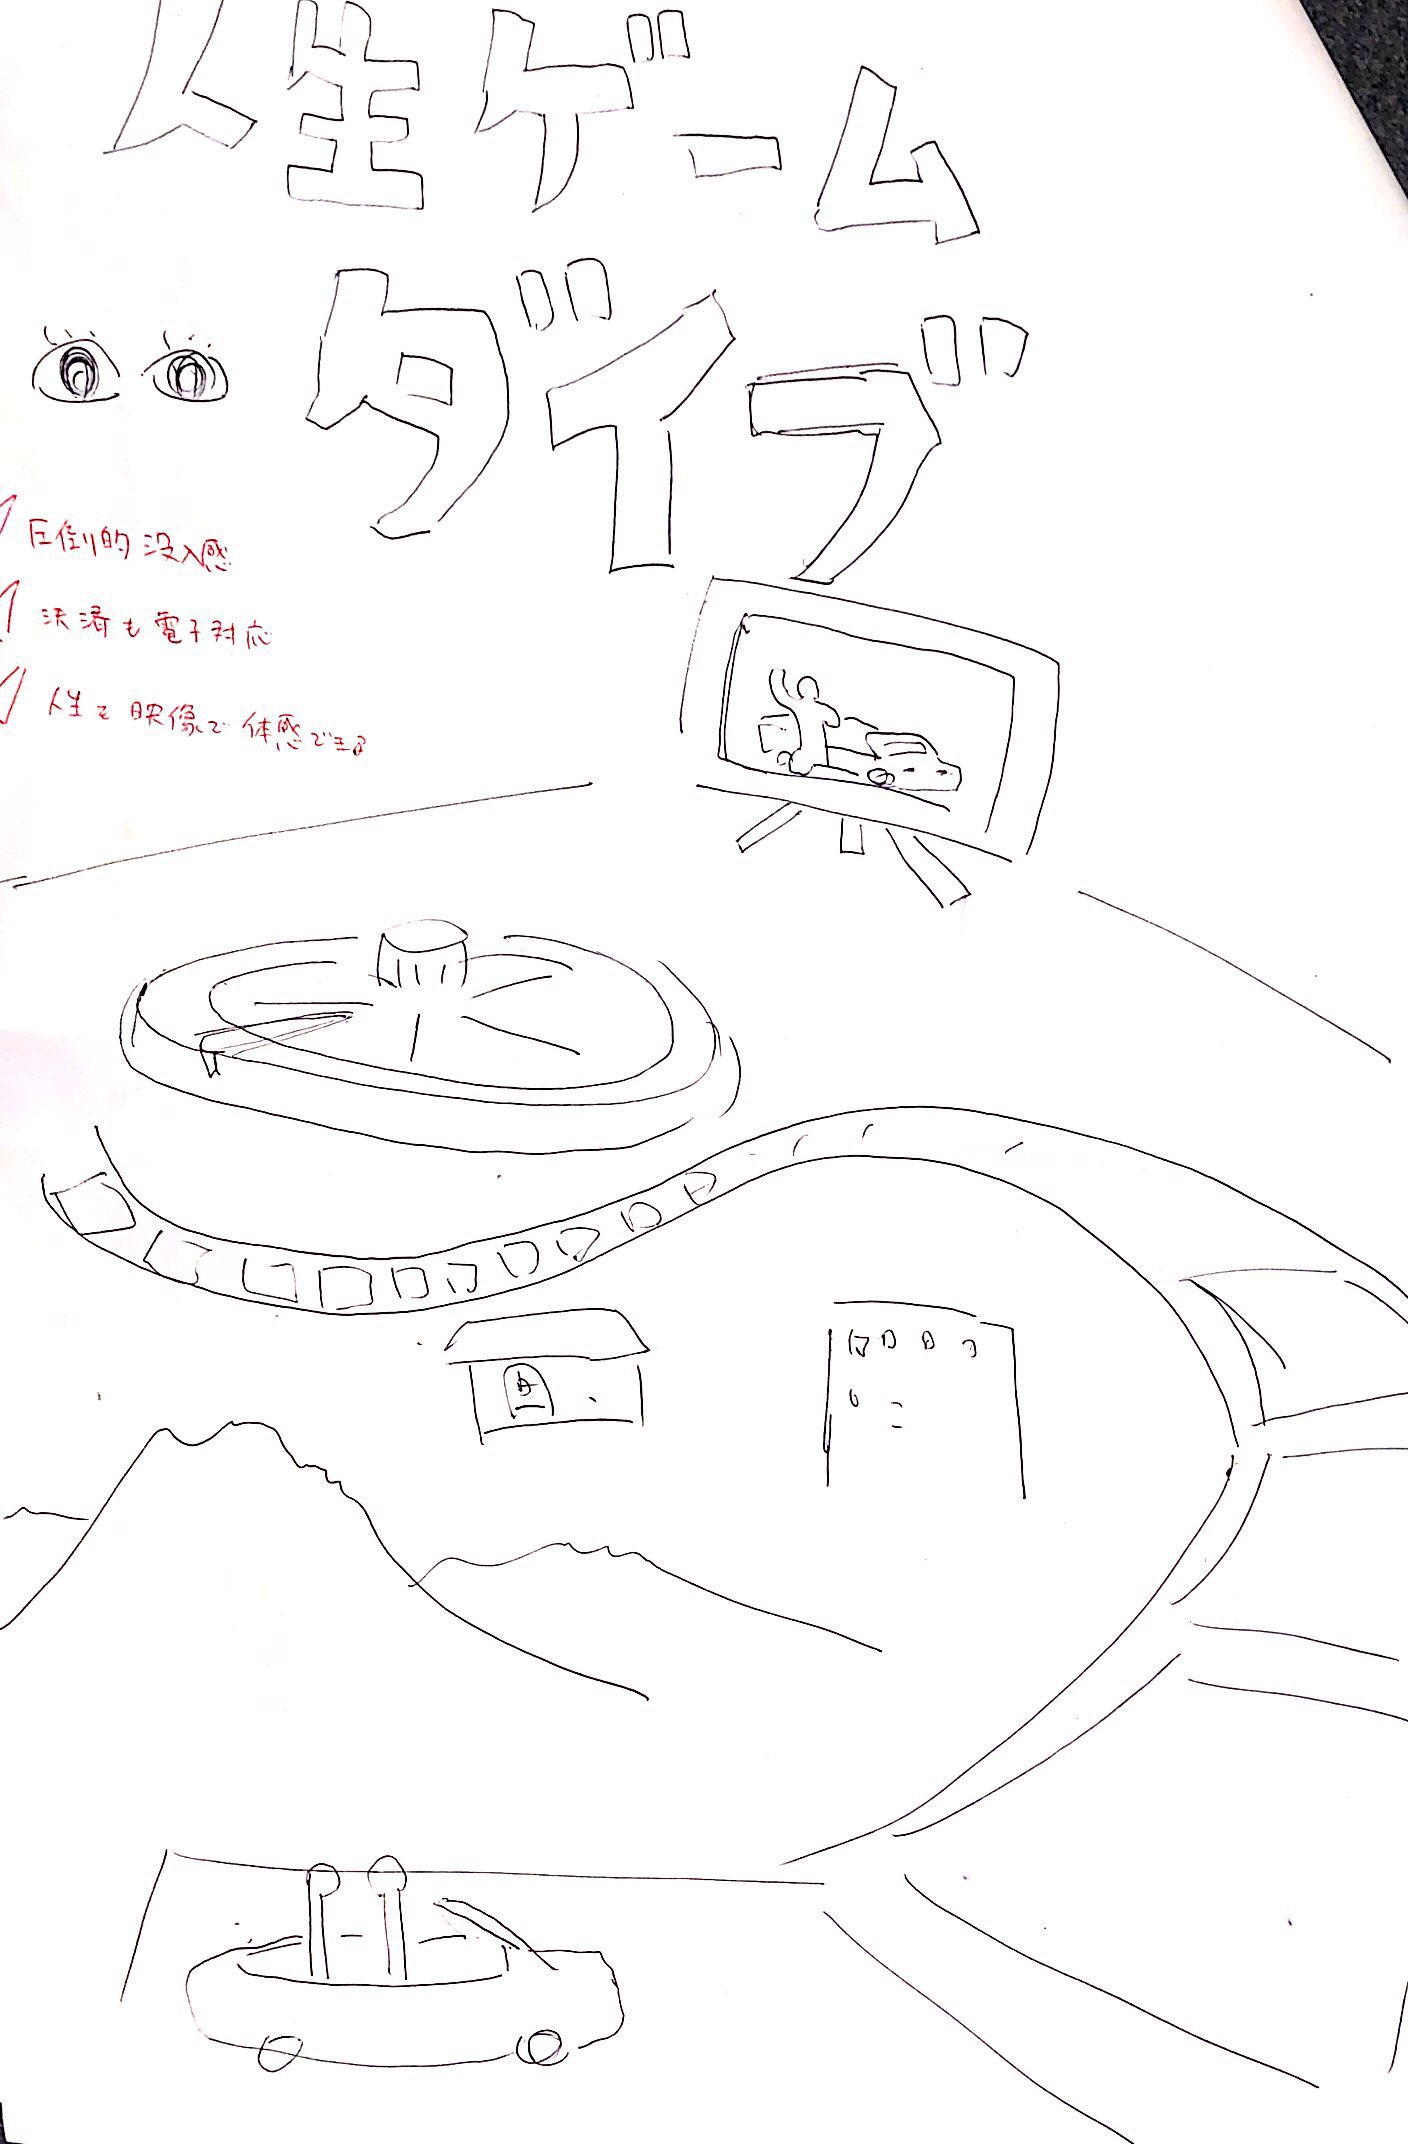
\includegraphics[width=50mm]{figures/group7.jpg}
 \end{center}
 \label{fig:seven}
 \end{minipage}
 \begin{minipage}{0.47\hsize}
 \begin{center}
 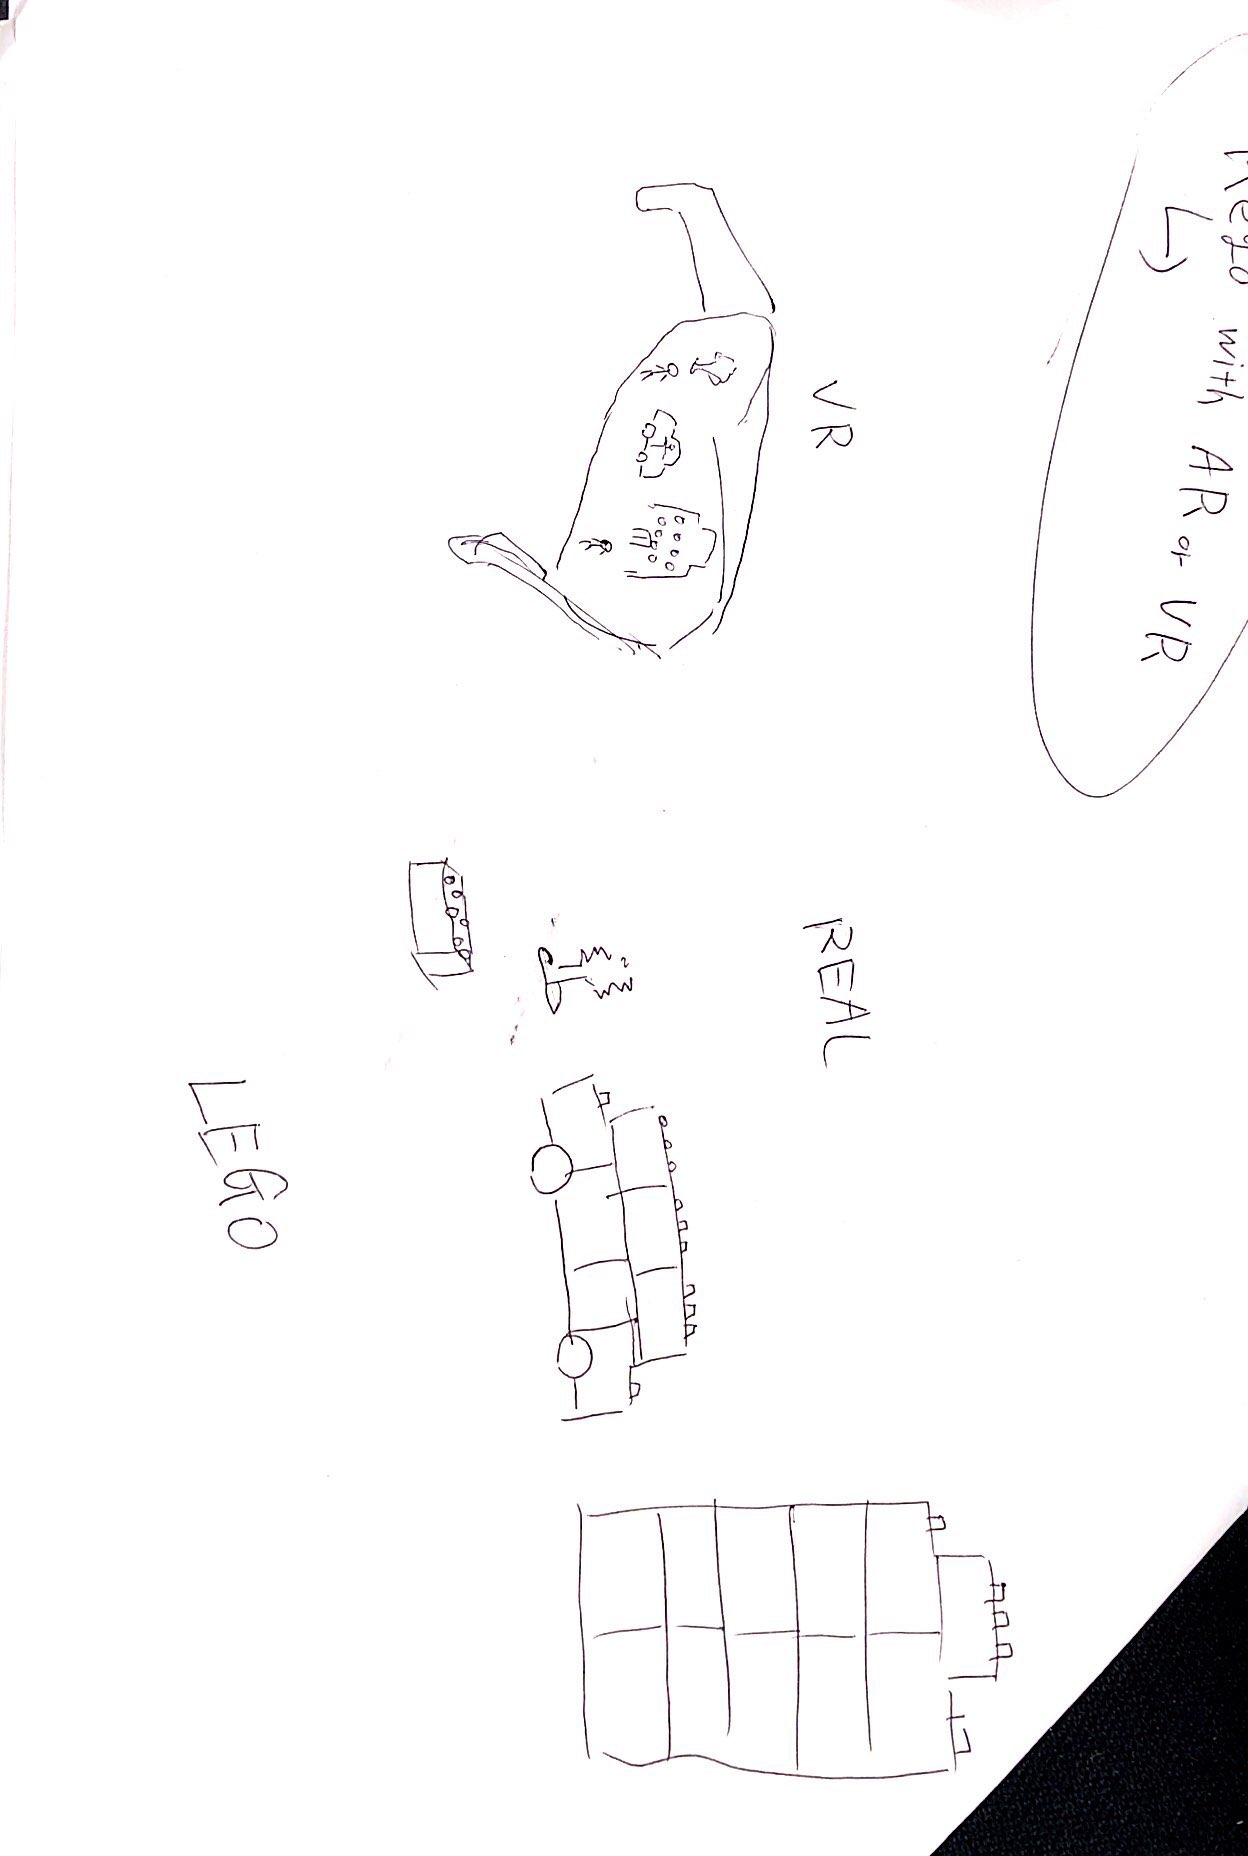
\includegraphics[width=50mm]{figures/group8.jpg}
 \end{center}
 \label{fig:eight}
 \end{minipage}
\end{figure}
\begin{figure}[H]
 \begin{minipage}{0.47\hsize}
 \begin{center}
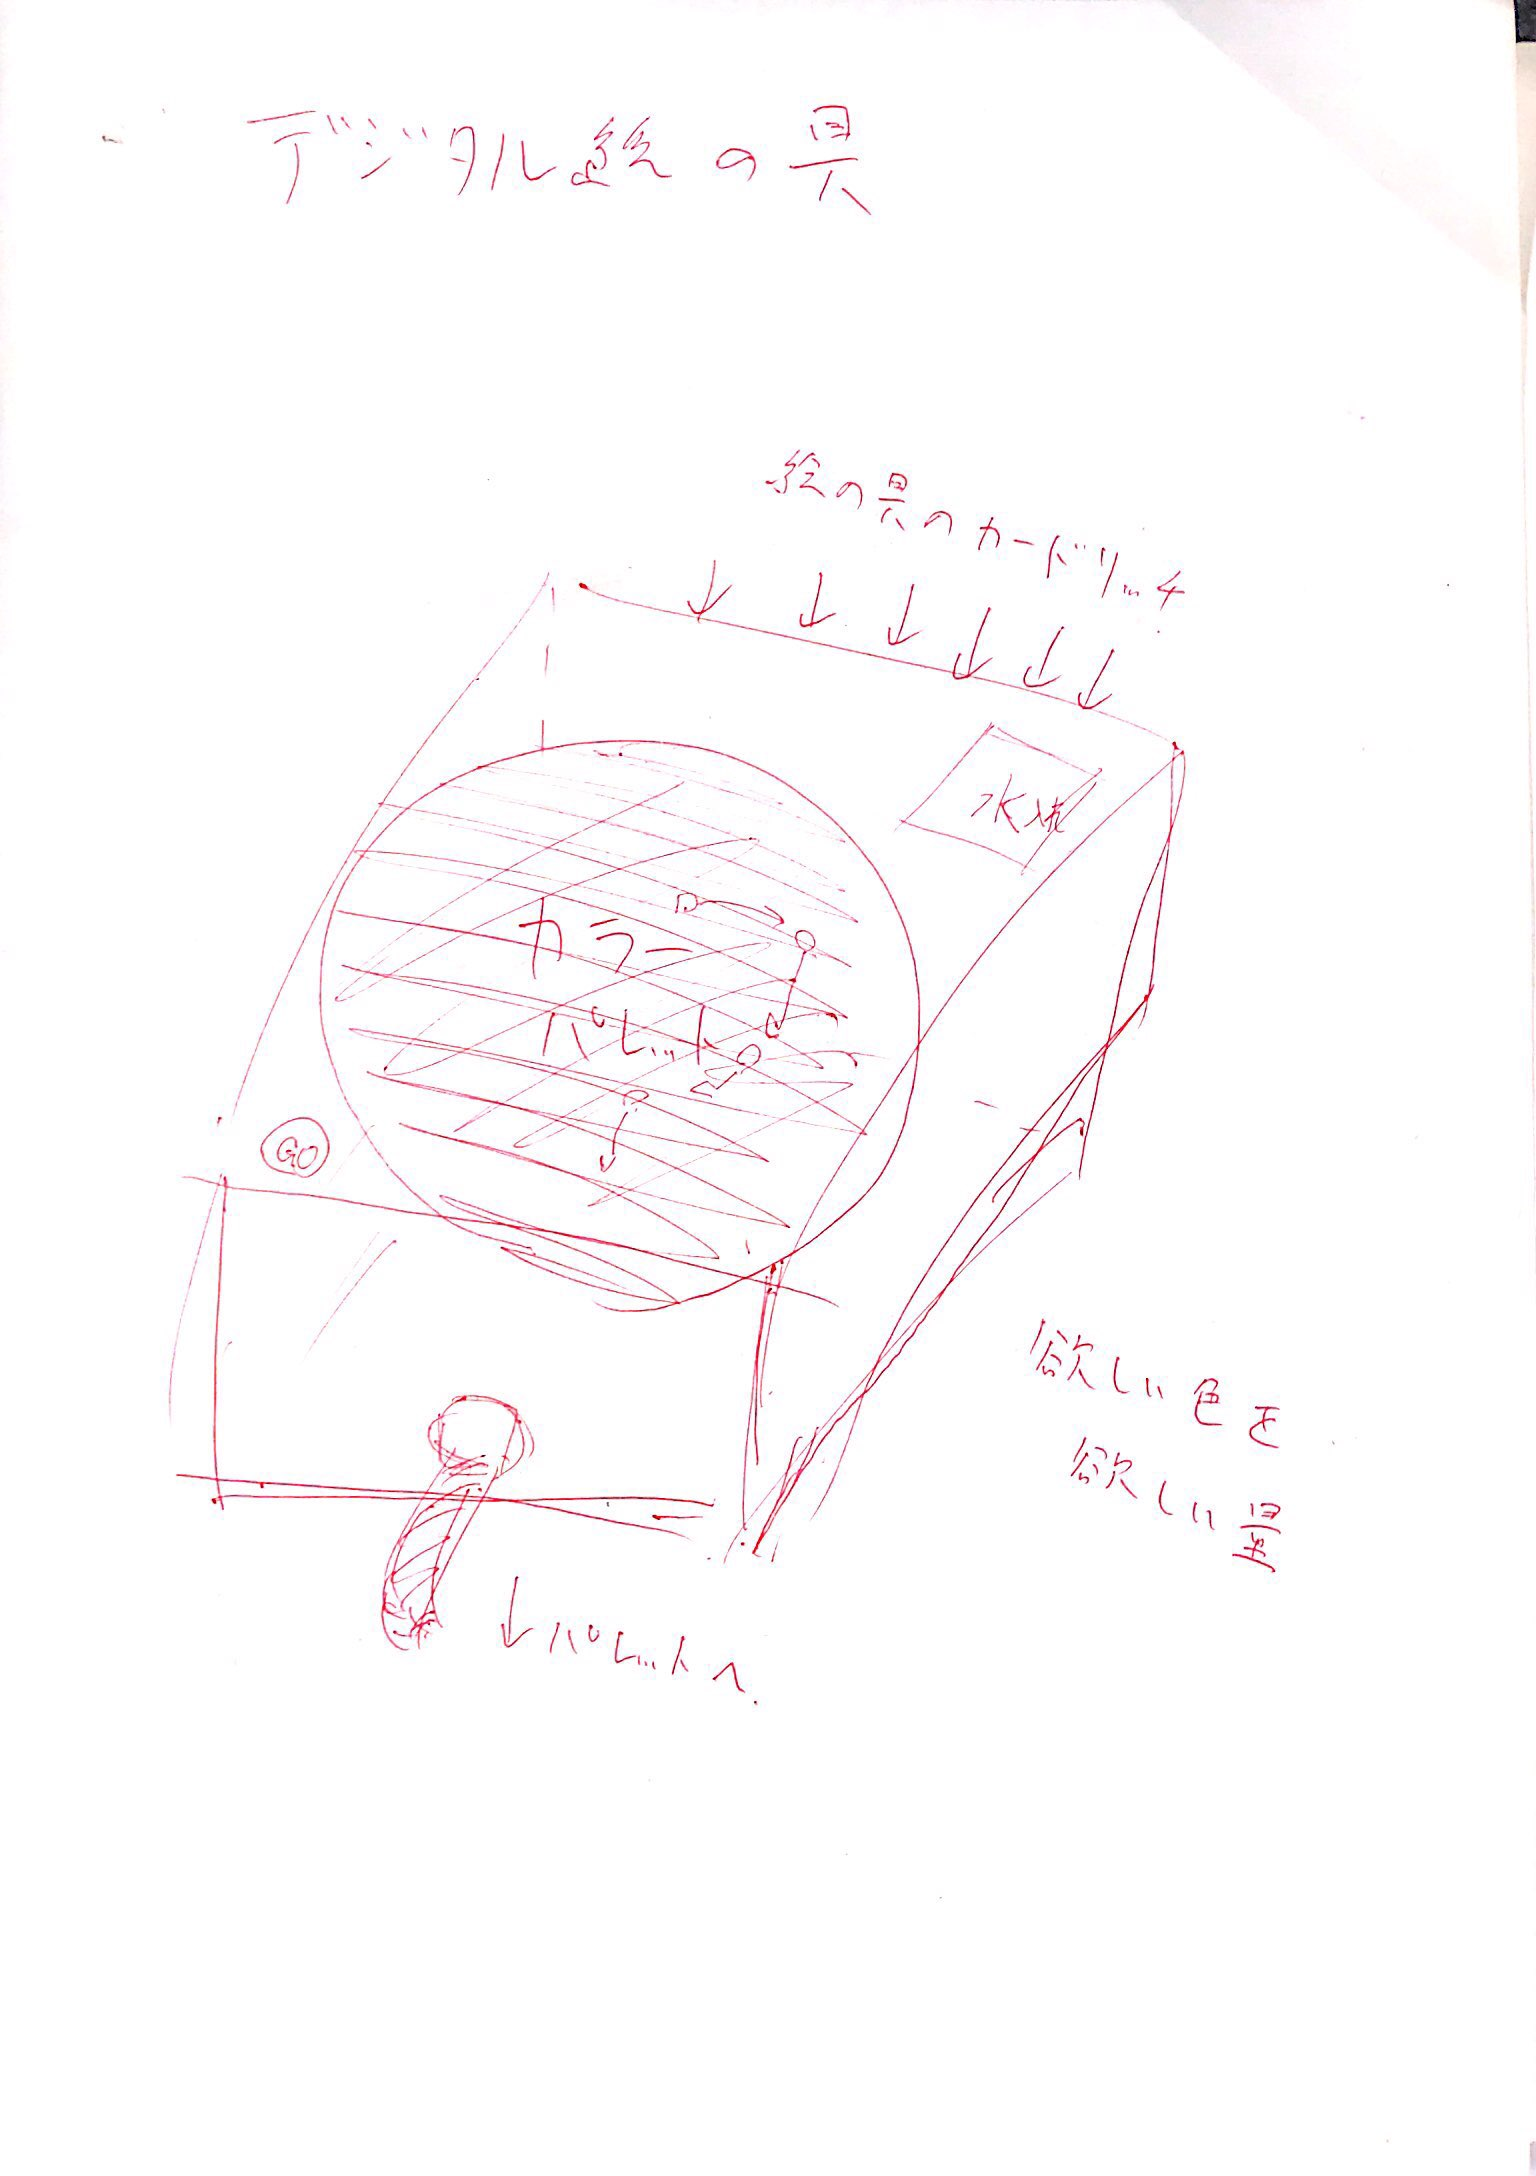
\includegraphics[width=50mm]{figures/group9.jpg}
 \end{center}
 \label{fig:seven}
 \end{minipage}
 \begin{minipage}{0.47\hsize}
 \begin{center}
 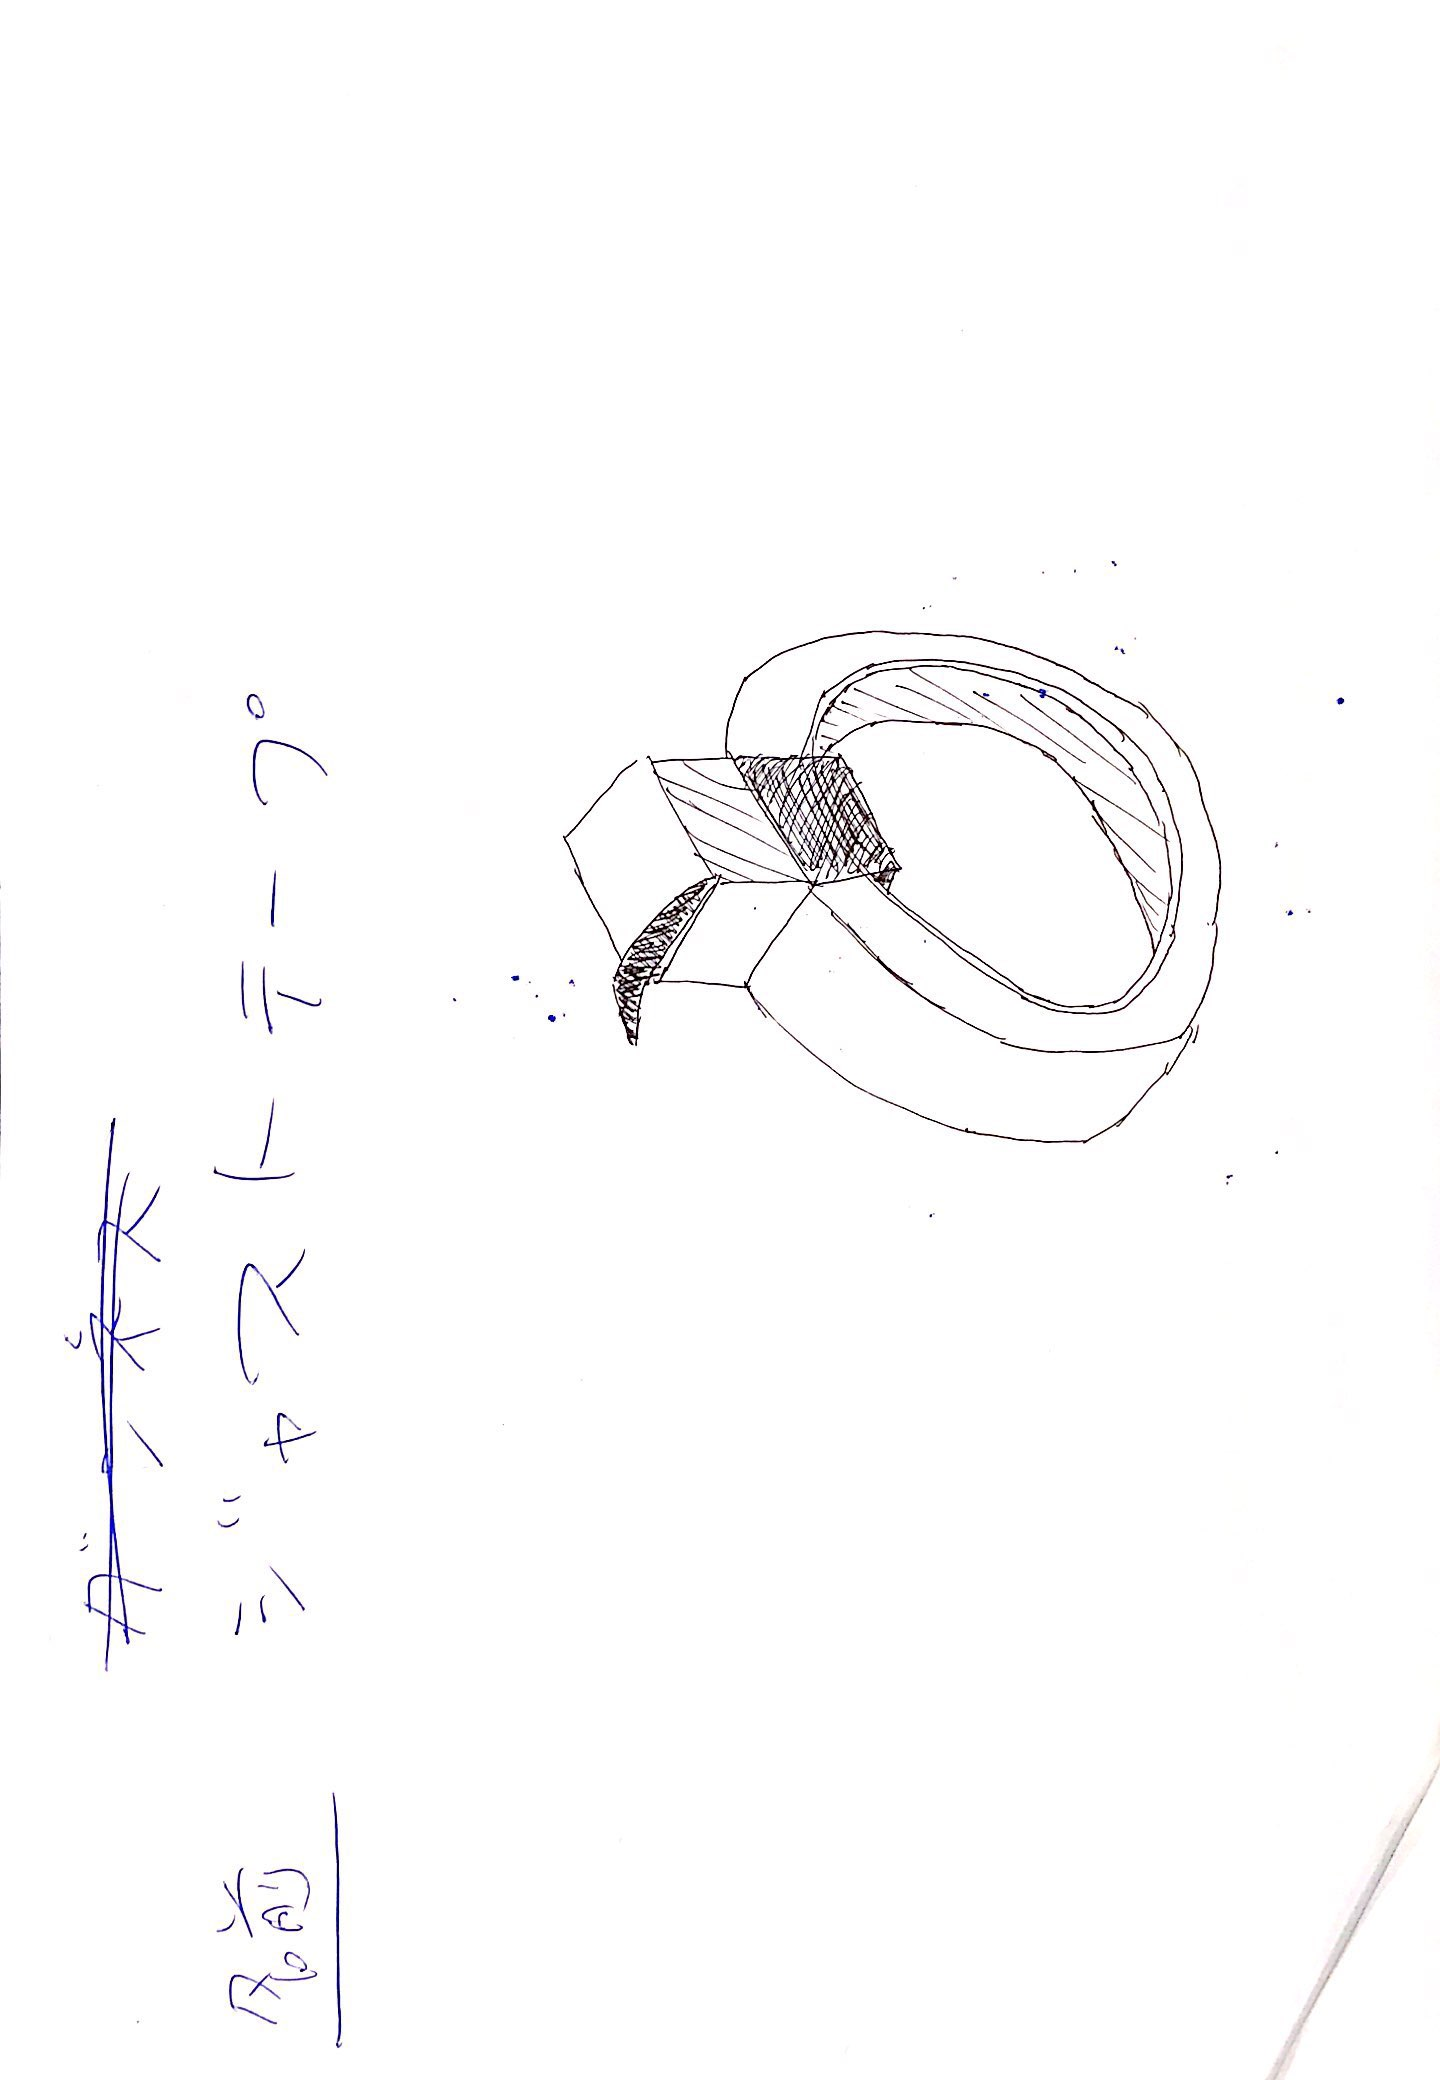
\includegraphics[width=50mm]{figures/group10.jpg}
 \end{center}
 \label{fig:eight}
 \end{minipage}
\end{figure}
\begin{figure}[H]
 \begin{minipage}{0.47\hsize}
 \begin{center}
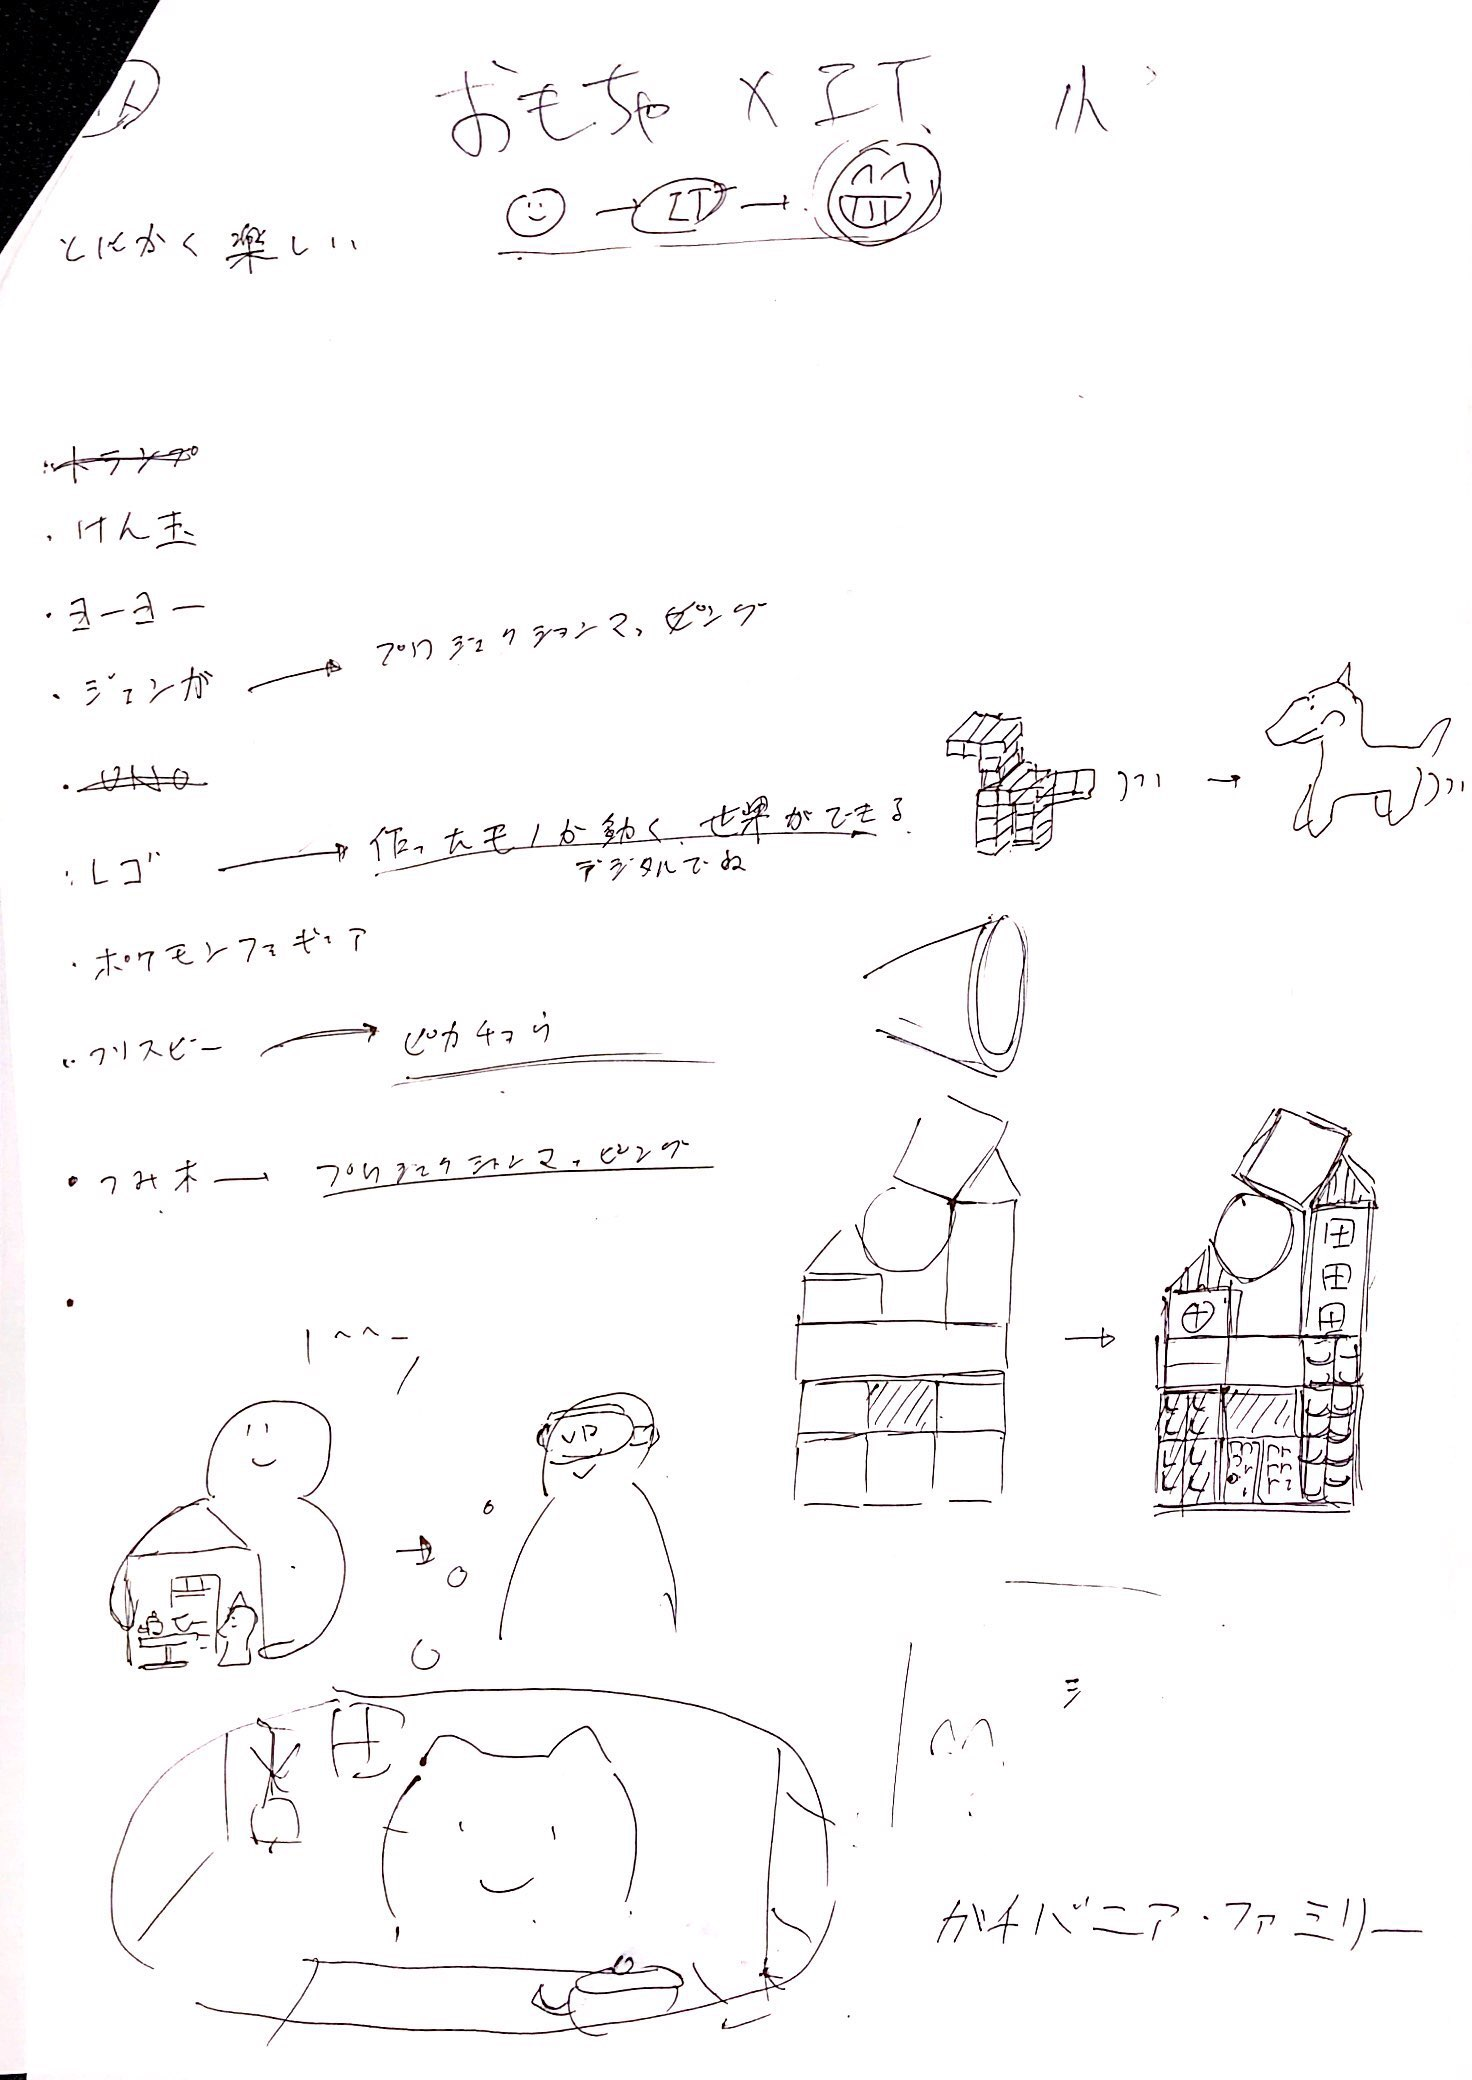
\includegraphics[width=50mm]{figures/group11.jpg}
 \end{center}
 \label{fig:seven}
 \end{minipage}
 \begin{minipage}{0.47\hsize}
 \begin{center}
 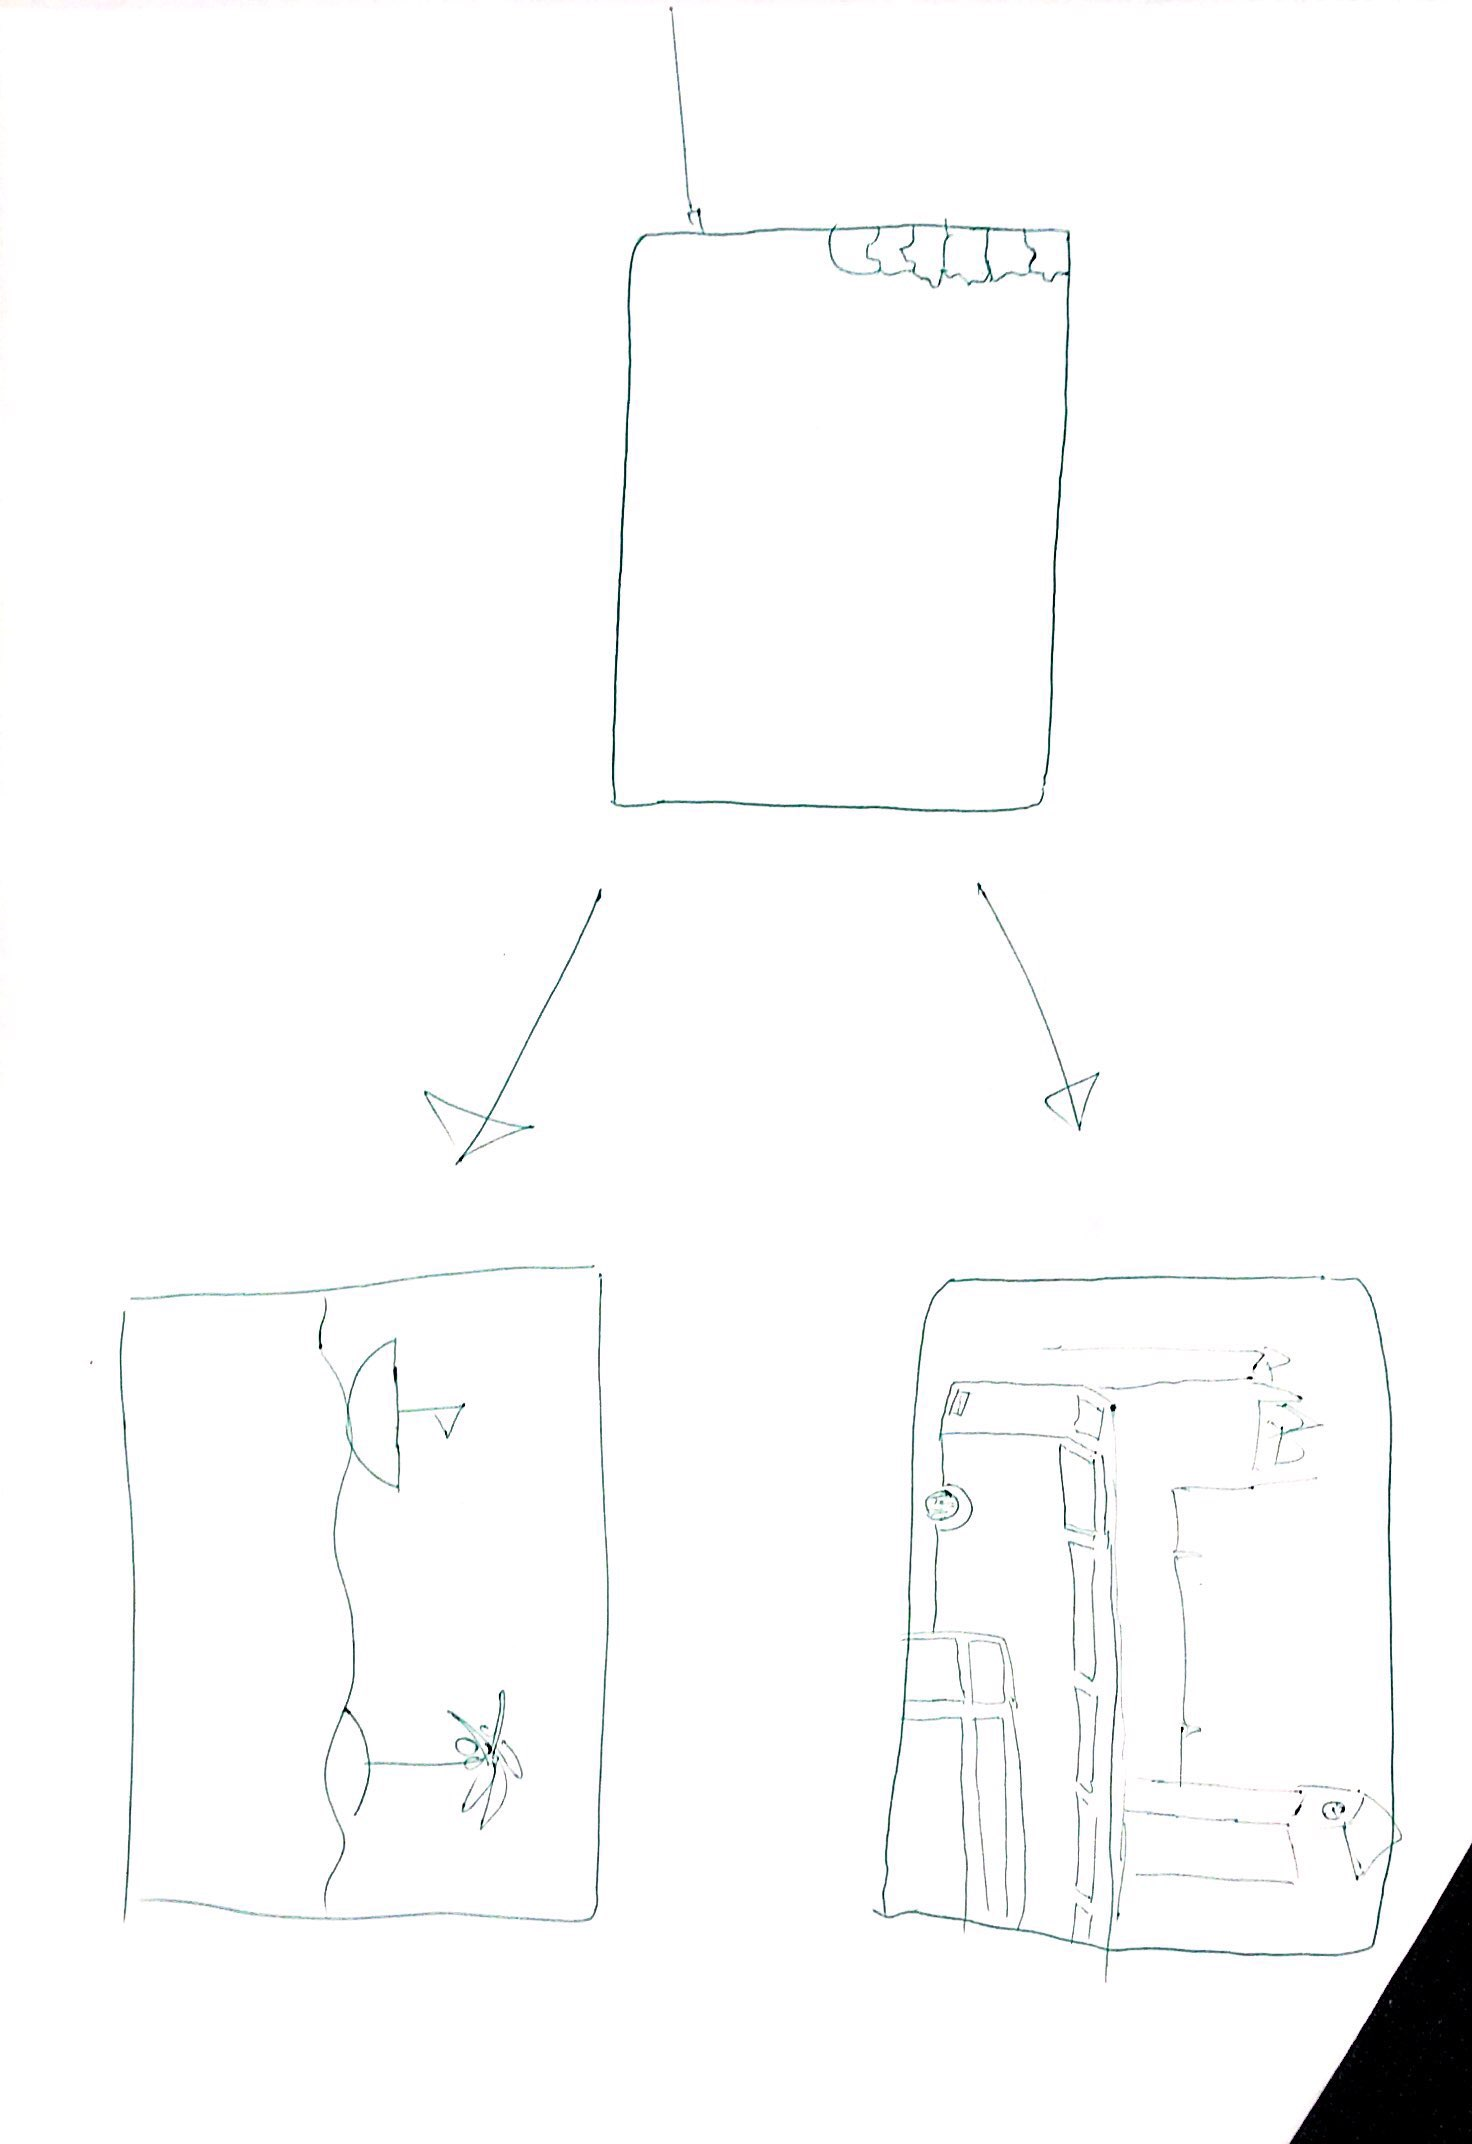
\includegraphics[width=50mm]{figures/group12.jpg}
 \end{center}
 \label{fig:eight}
 \end{minipage}
\end{figure}



%--------------------------------------------------------------------
% 図一覧
\listoffigures

%--------------------------------------------------------------------
% 表一覧
\listoftables

\end{document}
